% Options for packages loaded elsewhere
\PassOptionsToPackage{unicode}{hyperref}
\PassOptionsToPackage{hyphens}{url}
\PassOptionsToPackage{dvipsnames,svgnames,x11names}{xcolor}
%
\documentclass[
  letterpaper,
  DIV=11,
  numbers=noendperiod]{scrartcl}

\usepackage{amsmath,amssymb}
\usepackage{iftex}
\ifPDFTeX
  \usepackage[T1]{fontenc}
  \usepackage[utf8]{inputenc}
  \usepackage{textcomp} % provide euro and other symbols
\else % if luatex or xetex
  \usepackage{unicode-math}
  \defaultfontfeatures{Scale=MatchLowercase}
  \defaultfontfeatures[\rmfamily]{Ligatures=TeX,Scale=1}
\fi
\usepackage{lmodern}
\ifPDFTeX\else  
    % xetex/luatex font selection
\fi
% Use upquote if available, for straight quotes in verbatim environments
\IfFileExists{upquote.sty}{\usepackage{upquote}}{}
\IfFileExists{microtype.sty}{% use microtype if available
  \usepackage[]{microtype}
  \UseMicrotypeSet[protrusion]{basicmath} % disable protrusion for tt fonts
}{}
\makeatletter
\@ifundefined{KOMAClassName}{% if non-KOMA class
  \IfFileExists{parskip.sty}{%
    \usepackage{parskip}
  }{% else
    \setlength{\parindent}{0pt}
    \setlength{\parskip}{6pt plus 2pt minus 1pt}}
}{% if KOMA class
  \KOMAoptions{parskip=half}}
\makeatother
\usepackage{xcolor}
\setlength{\emergencystretch}{3em} % prevent overfull lines
\setcounter{secnumdepth}{-\maxdimen} % remove section numbering
% Make \paragraph and \subparagraph free-standing
\ifx\paragraph\undefined\else
  \let\oldparagraph\paragraph
  \renewcommand{\paragraph}[1]{\oldparagraph{#1}\mbox{}}
\fi
\ifx\subparagraph\undefined\else
  \let\oldsubparagraph\subparagraph
  \renewcommand{\subparagraph}[1]{\oldsubparagraph{#1}\mbox{}}
\fi

\usepackage{color}
\usepackage{fancyvrb}
\newcommand{\VerbBar}{|}
\newcommand{\VERB}{\Verb[commandchars=\\\{\}]}
\DefineVerbatimEnvironment{Highlighting}{Verbatim}{commandchars=\\\{\}}
% Add ',fontsize=\small' for more characters per line
\usepackage{framed}
\definecolor{shadecolor}{RGB}{241,243,245}
\newenvironment{Shaded}{\begin{snugshade}}{\end{snugshade}}
\newcommand{\AlertTok}[1]{\textcolor[rgb]{0.68,0.00,0.00}{#1}}
\newcommand{\AnnotationTok}[1]{\textcolor[rgb]{0.37,0.37,0.37}{#1}}
\newcommand{\AttributeTok}[1]{\textcolor[rgb]{0.40,0.45,0.13}{#1}}
\newcommand{\BaseNTok}[1]{\textcolor[rgb]{0.68,0.00,0.00}{#1}}
\newcommand{\BuiltInTok}[1]{\textcolor[rgb]{0.00,0.23,0.31}{#1}}
\newcommand{\CharTok}[1]{\textcolor[rgb]{0.13,0.47,0.30}{#1}}
\newcommand{\CommentTok}[1]{\textcolor[rgb]{0.37,0.37,0.37}{#1}}
\newcommand{\CommentVarTok}[1]{\textcolor[rgb]{0.37,0.37,0.37}{\textit{#1}}}
\newcommand{\ConstantTok}[1]{\textcolor[rgb]{0.56,0.35,0.01}{#1}}
\newcommand{\ControlFlowTok}[1]{\textcolor[rgb]{0.00,0.23,0.31}{#1}}
\newcommand{\DataTypeTok}[1]{\textcolor[rgb]{0.68,0.00,0.00}{#1}}
\newcommand{\DecValTok}[1]{\textcolor[rgb]{0.68,0.00,0.00}{#1}}
\newcommand{\DocumentationTok}[1]{\textcolor[rgb]{0.37,0.37,0.37}{\textit{#1}}}
\newcommand{\ErrorTok}[1]{\textcolor[rgb]{0.68,0.00,0.00}{#1}}
\newcommand{\ExtensionTok}[1]{\textcolor[rgb]{0.00,0.23,0.31}{#1}}
\newcommand{\FloatTok}[1]{\textcolor[rgb]{0.68,0.00,0.00}{#1}}
\newcommand{\FunctionTok}[1]{\textcolor[rgb]{0.28,0.35,0.67}{#1}}
\newcommand{\ImportTok}[1]{\textcolor[rgb]{0.00,0.46,0.62}{#1}}
\newcommand{\InformationTok}[1]{\textcolor[rgb]{0.37,0.37,0.37}{#1}}
\newcommand{\KeywordTok}[1]{\textcolor[rgb]{0.00,0.23,0.31}{#1}}
\newcommand{\NormalTok}[1]{\textcolor[rgb]{0.00,0.23,0.31}{#1}}
\newcommand{\OperatorTok}[1]{\textcolor[rgb]{0.37,0.37,0.37}{#1}}
\newcommand{\OtherTok}[1]{\textcolor[rgb]{0.00,0.23,0.31}{#1}}
\newcommand{\PreprocessorTok}[1]{\textcolor[rgb]{0.68,0.00,0.00}{#1}}
\newcommand{\RegionMarkerTok}[1]{\textcolor[rgb]{0.00,0.23,0.31}{#1}}
\newcommand{\SpecialCharTok}[1]{\textcolor[rgb]{0.37,0.37,0.37}{#1}}
\newcommand{\SpecialStringTok}[1]{\textcolor[rgb]{0.13,0.47,0.30}{#1}}
\newcommand{\StringTok}[1]{\textcolor[rgb]{0.13,0.47,0.30}{#1}}
\newcommand{\VariableTok}[1]{\textcolor[rgb]{0.07,0.07,0.07}{#1}}
\newcommand{\VerbatimStringTok}[1]{\textcolor[rgb]{0.13,0.47,0.30}{#1}}
\newcommand{\WarningTok}[1]{\textcolor[rgb]{0.37,0.37,0.37}{\textit{#1}}}

\providecommand{\tightlist}{%
  \setlength{\itemsep}{0pt}\setlength{\parskip}{0pt}}\usepackage{longtable,booktabs,array}
\usepackage{calc} % for calculating minipage widths
% Correct order of tables after \paragraph or \subparagraph
\usepackage{etoolbox}
\makeatletter
\patchcmd\longtable{\par}{\if@noskipsec\mbox{}\fi\par}{}{}
\makeatother
% Allow footnotes in longtable head/foot
\IfFileExists{footnotehyper.sty}{\usepackage{footnotehyper}}{\usepackage{footnote}}
\makesavenoteenv{longtable}
\usepackage{graphicx}
\makeatletter
\def\maxwidth{\ifdim\Gin@nat@width>\linewidth\linewidth\else\Gin@nat@width\fi}
\def\maxheight{\ifdim\Gin@nat@height>\textheight\textheight\else\Gin@nat@height\fi}
\makeatother
% Scale images if necessary, so that they will not overflow the page
% margins by default, and it is still possible to overwrite the defaults
% using explicit options in \includegraphics[width, height, ...]{}
\setkeys{Gin}{width=\maxwidth,height=\maxheight,keepaspectratio}
% Set default figure placement to htbp
\makeatletter
\def\fps@figure{htbp}
\makeatother

\KOMAoption{captions}{tableheading}
\makeatletter
\makeatother
\makeatletter
\makeatother
\makeatletter
\@ifpackageloaded{caption}{}{\usepackage{caption}}
\AtBeginDocument{%
\ifdefined\contentsname
  \renewcommand*\contentsname{Table of contents}
\else
  \newcommand\contentsname{Table of contents}
\fi
\ifdefined\listfigurename
  \renewcommand*\listfigurename{List of Figures}
\else
  \newcommand\listfigurename{List of Figures}
\fi
\ifdefined\listtablename
  \renewcommand*\listtablename{List of Tables}
\else
  \newcommand\listtablename{List of Tables}
\fi
\ifdefined\figurename
  \renewcommand*\figurename{Figure}
\else
  \newcommand\figurename{Figure}
\fi
\ifdefined\tablename
  \renewcommand*\tablename{Table}
\else
  \newcommand\tablename{Table}
\fi
}
\@ifpackageloaded{float}{}{\usepackage{float}}
\floatstyle{ruled}
\@ifundefined{c@chapter}{\newfloat{codelisting}{h}{lop}}{\newfloat{codelisting}{h}{lop}[chapter]}
\floatname{codelisting}{Listing}
\newcommand*\listoflistings{\listof{codelisting}{List of Listings}}
\makeatother
\makeatletter
\@ifpackageloaded{caption}{}{\usepackage{caption}}
\@ifpackageloaded{subcaption}{}{\usepackage{subcaption}}
\makeatother
\makeatletter
\@ifpackageloaded{tcolorbox}{}{\usepackage[skins,breakable]{tcolorbox}}
\makeatother
\makeatletter
\@ifundefined{shadecolor}{\definecolor{shadecolor}{rgb}{.97, .97, .97}}
\makeatother
\makeatletter
\makeatother
\makeatletter
\makeatother
\ifLuaTeX
  \usepackage{selnolig}  % disable illegal ligatures
\fi
\IfFileExists{bookmark.sty}{\usepackage{bookmark}}{\usepackage{hyperref}}
\IfFileExists{xurl.sty}{\usepackage{xurl}}{} % add URL line breaks if available
\urlstyle{same} % disable monospaced font for URLs
\hypersetup{
  pdftitle={The Grammar of Graphics},
  pdfauthor={Gabriel I. Cook},
  colorlinks=true,
  linkcolor={blue},
  filecolor={Maroon},
  citecolor={Blue},
  urlcolor={Blue},
  pdfcreator={LaTeX via pandoc}}

\title{\textbf{The Grammar of Graphics}}
\author{Gabriel I. Cook}
\date{2023-06-28}

\begin{document}
\maketitle
\ifdefined\Shaded\renewenvironment{Shaded}{\begin{tcolorbox}[boxrule=0pt, sharp corners, interior hidden, borderline west={3pt}{0pt}{shadecolor}, breakable, enhanced, frame hidden]}{\end{tcolorbox}}\fi

\hypertarget{section}{%
\section{}\label{section}}

\begin{Shaded}
\begin{Highlighting}[]
\FunctionTok{library}\NormalTok{(magrittr)}
\FunctionTok{library}\NormalTok{(dplyr)}
\end{Highlighting}
\end{Shaded}

\begin{verbatim}

Attaching package: 'dplyr'
\end{verbatim}

\begin{verbatim}
The following objects are masked from 'package:stats':

    filter, lag
\end{verbatim}

\begin{verbatim}
The following objects are masked from 'package:base':

    intersect, setdiff, setequal, union
\end{verbatim}

\begin{Shaded}
\begin{Highlighting}[]
\FunctionTok{library}\NormalTok{(ggplot2)}

\NormalTok{quick\_data }\OtherTok{\textless{}{-}} \FunctionTok{data.frame}\NormalTok{(}
  \AttributeTok{A =} \FunctionTok{c}\NormalTok{(}\StringTok{"Male"}\NormalTok{, }\StringTok{"Male"}\NormalTok{, }\StringTok{"Female"}\NormalTok{, }\StringTok{"Female"}\NormalTok{, }\ConstantTok{NA}\NormalTok{),}
  \AttributeTok{B =} \FunctionTok{c}\NormalTok{(}\DecValTok{1}\NormalTok{, }\DecValTok{0}\NormalTok{, }\DecValTok{1}\NormalTok{, }\DecValTok{0}\NormalTok{, }\ConstantTok{NA}\NormalTok{),}
  \AttributeTok{C =} \FunctionTok{c}\NormalTok{(}\DecValTok{1}\NormalTok{, }\DecValTok{5}\NormalTok{, }\DecValTok{6}\NormalTok{, }\DecValTok{3}\NormalTok{, }\ConstantTok{NA}\NormalTok{)}
\NormalTok{) }

\NormalTok{quick\_data }\SpecialCharTok{\%\textgreater{}\%} 
  \FunctionTok{mutate}\NormalTok{(., }\AttributeTok{J =} \FunctionTok{case\_when}\NormalTok{(A }\SpecialCharTok{==} \StringTok{"Male"} \SpecialCharTok{\textasciitilde{}} \StringTok{"a"}\NormalTok{, }\ConstantTok{TRUE} \SpecialCharTok{\textasciitilde{}} \StringTok{"b"}\NormalTok{))}
\end{Highlighting}
\end{Shaded}

\begin{verbatim}
       A  B  C J
1   Male  1  1 a
2   Male  0  5 a
3 Female  1  6 b
4 Female  0  3 b
5   <NA> NA NA b
\end{verbatim}

\begin{Shaded}
\begin{Highlighting}[]
\FunctionTok{ggplot}\NormalTok{(}\AttributeTok{data =}\NormalTok{ quick\_data) }\SpecialCharTok{+}
  \FunctionTok{geom\_point}\NormalTok{(}\FunctionTok{aes}\NormalTok{(B, C), }\AttributeTok{color =} \StringTok{"blue"}\NormalTok{)}
\end{Highlighting}
\end{Shaded}

\begin{verbatim}
Warning: Removed 1 rows containing missing values (`geom_point()`).
\end{verbatim}

\begin{figure}[H]

{\centering 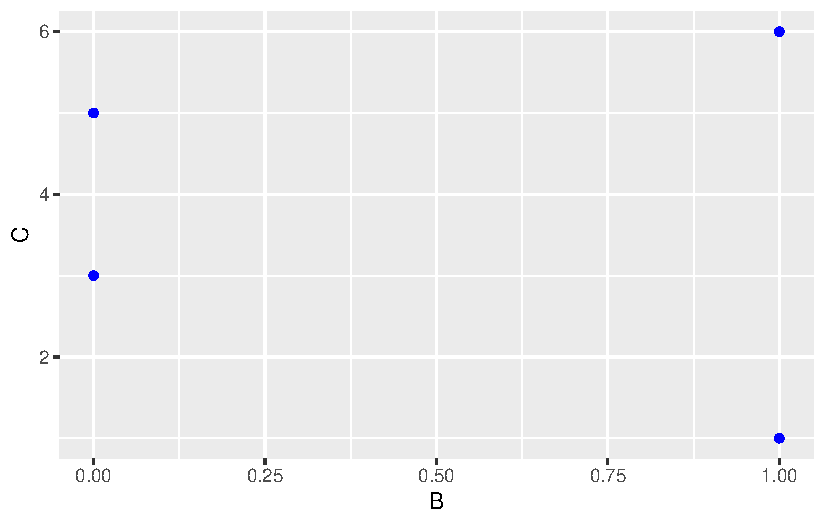
\includegraphics{Intro_to__ggplot_files/figure-pdf/unnamed-chunk-1-1.pdf}

}

\end{figure}

\begin{Shaded}
\begin{Highlighting}[]
\NormalTok{mydata }\OtherTok{\textless{}{-}} \FunctionTok{data.frame}\NormalTok{(}
  \AttributeTok{A =} \FunctionTok{c}\NormalTok{(}\StringTok{"Male"}\NormalTok{, }\StringTok{"Male"}\NormalTok{, }\StringTok{"Female"}\NormalTok{, }\StringTok{"Female"}\NormalTok{, }\ConstantTok{NA}\NormalTok{),}
  \AttributeTok{B =} \FunctionTok{c}\NormalTok{(}\DecValTok{1}\NormalTok{, }\DecValTok{2}\NormalTok{, }\DecValTok{10}\NormalTok{, }\DecValTok{30}\NormalTok{, }\ConstantTok{NA}\NormalTok{),}
  \AttributeTok{C =} \FunctionTok{c}\NormalTok{(}\DecValTok{1}\NormalTok{, }\DecValTok{5}\NormalTok{, }\DecValTok{6}\NormalTok{, }\DecValTok{3}\NormalTok{, }\ConstantTok{NA}\NormalTok{)}
\NormalTok{)  }
\end{Highlighting}
\end{Shaded}

Integrate the label changes for factors and levels:

guides(fill = guide\_legend(title = ``my title''))
scale\_fill\_discrete(``Color 1'', ``Color 2'') To plot means.
stat\_summary(fun = ``mean'', geom = ``col'')

compute mean and sd and then pass to geom\_errorbar()

\hypertarget{overview}{%
\section{\texorpdfstring{\textbf{Overview}}{Overview}}\label{overview}}

Data visualization is key to understanding data. This exercise will use
\texttt{dplyr} most prominently. Piecing together the components will be
difficult but in the end you need visualizations. At very least you
should gain an understanding of chaining functions together in
\texttt{dplyr} using the \texttt{\%\textgreater{}\%} from the
\texttt{magrittr} library in order to set by step manipulate a data
frame.

Some Helpful Functions:

\begin{itemize}
\tightlist
\item
  \texttt{ggplot()}: for initializing a plot object
\item
  \texttt{aes()}: for specifying aesthetics of a plot (e.g., x, y, size,
  color, etc.)
\item
  \texttt{geom\_bar()}: for bar geometry of a plot using either x or y
\item
  \texttt{geom\_col()}: for bar geometry of a plot using x and y
\item
  \texttt{geom\_point()}: for point geometry of a plot
\item
  \texttt{geom\_line()}: for line geometry of a plot
\item
  \texttt{geom\_histogram()}: for a distribution geometry of a plot
\item
  \texttt{ggtitle()} or \texttt{labs()}: for adding a title
\item
  \texttt{geom\_text()}: for editing text
\item
  \texttt{ylab()} and \texttt{xlab()}: for axis labeling
\item
  \texttt{coord\_flip()}: for flipping the x and y coordinates\\
\item
  \texttt{theme\_minimal()}: a particular theme application
\item
  \texttt{theme\_set()}: for setting a theme
\end{itemize}

\hypertarget{loading-libraries}{%
\section{\texorpdfstring{\textbf{Loading
Libraries}}{Loading Libraries}}\label{loading-libraries}}

You will need to load \texttt{dplyr} and \texttt{ggplot2}.

\begin{Shaded}
\begin{Highlighting}[]
\FunctionTok{library}\NormalTok{(ggplot2)}
\FunctionTok{library}\NormalTok{(dplyr)}
\FunctionTok{library}\NormalTok{(magrittr)}
\end{Highlighting}
\end{Shaded}

\hypertarget{example-an-xy-scatterplot}{%
\section{\texorpdfstring{\textbf{Example: An XY
Scatterplot}}{Example: An XY Scatterplot}}\label{example-an-xy-scatterplot}}

Here is an example of a scatterplot communicating the relationship
between \texttt{mpg} and \texttt{cyl} (cylinder size) from the
\texttt{mtcars} data set. The plot uses two data frames, one of which
summarizes the \texttt{mpg} means for each \texttt{cyl} level. Yes, you
can use two data frames in the same plot.

\begin{Shaded}
\begin{Highlighting}[]
\NormalTok{mt\_means }\OtherTok{\textless{}{-}}\NormalTok{ mtcars }\SpecialCharTok{\%\textgreater{}\%} \FunctionTok{group\_by}\NormalTok{(., cyl) }\SpecialCharTok{\%\textgreater{}\%} \FunctionTok{summarise}\NormalTok{(., }\AttributeTok{mean =} \FunctionTok{mean}\NormalTok{(mpg))}

\FunctionTok{ggplot}\NormalTok{(mtcars) }\SpecialCharTok{+}
  \FunctionTok{geom\_point}\NormalTok{(}\FunctionTok{aes}\NormalTok{(}\AttributeTok{x =} \FunctionTok{factor}\NormalTok{(cyl), }
                 \AttributeTok{y =}\NormalTok{ mpg, }
                 \AttributeTok{color =} \FunctionTok{factor}\NormalTok{(cyl)),}
             \AttributeTok{shape =} \DecValTok{22}\NormalTok{, }\AttributeTok{position =} \StringTok{"jitter"}\NormalTok{) }\SpecialCharTok{+} 
  \FunctionTok{geom\_point}\NormalTok{(}\AttributeTok{data =}\NormalTok{ mt\_means, }
             \AttributeTok{mapping =} \FunctionTok{aes}\NormalTok{(}\AttributeTok{x =} \FunctionTok{factor}\NormalTok{(cyl),}
                           \AttributeTok{y =}\NormalTok{ mean,}
                           \AttributeTok{color =} \FunctionTok{factor}\NormalTok{(cyl)),}
             \AttributeTok{alpha =}\NormalTok{ .}\DecValTok{60}\NormalTok{,}
             \AttributeTok{size =} \DecValTok{3}\NormalTok{) }\SpecialCharTok{+}
  \FunctionTok{labs}\NormalTok{(}\AttributeTok{title =} \StringTok{"Relationship between Cylinder and MPG"}\NormalTok{) }\SpecialCharTok{+}
  \FunctionTok{xlab}\NormalTok{(}\StringTok{"Cylinder"}\NormalTok{) }\SpecialCharTok{+}
  \FunctionTok{ylab}\NormalTok{(}\StringTok{"Miles Per Gallon"}\NormalTok{) }\SpecialCharTok{+}
  \FunctionTok{scale\_color\_discrete}\NormalTok{(}\AttributeTok{name =} \StringTok{"Cylinders"}\NormalTok{,}
                       \CommentTok{\#breaks = c(8,6,4),}
                       \AttributeTok{labels =} \FunctionTok{c}\NormalTok{(}\StringTok{"8 Cylinder"}\NormalTok{,}\StringTok{"6 Cylinder"}\NormalTok{,}\StringTok{"4 Cylinder"}\NormalTok{)) }\SpecialCharTok{+}
\NormalTok{  see}\SpecialCharTok{::}\FunctionTok{theme\_modern}\NormalTok{()}
\end{Highlighting}
\end{Shaded}

\begin{figure}[H]

{\centering 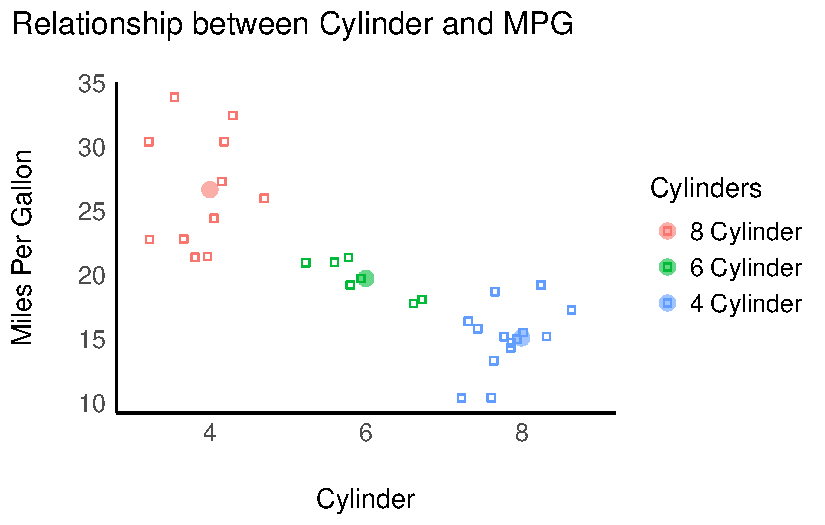
\includegraphics{Intro_to__ggplot_files/figure-pdf/unnamed-chunk-3-1.pdf}

}

\end{figure}

\hypertarget{the-grammar-of-graphics}{%
\section{\texorpdfstring{\textbf{The Grammar of
Graphics}}{The Grammar of Graphics}}\label{the-grammar-of-graphics}}

In {[}\emph{The Grammar of Graphics} (Wilkinson, 2005){]}
(https://www.amazon.com/Grammar-Graphics-Statistics-Computing/dp/0387245448),
Wilkinson explains how graphics can be created using layers that build
upon each other.

Plot layers build, starting with data:

\begin{itemize}
\tightlist
\item
  theme
\item
  coordinates
\item
  statistics
\item
  facets
\item
  geometries
\item
  aesthetics
\item
  data
\end{itemize}

\hypertarget{ggplot-plot-basics}{%
\section{\texorpdfstring{\textbf{\texttt{ggplot} Plot
Basics}}{ggplot Plot Basics}}\label{ggplot-plot-basics}}

\texttt{ggplot2} was created based on Wilkinsons's grammar structure, so
all plots using \texttt{ggplot2} start with a base foundation, on top
which layers are added according to their own aesthetic attributes.

As Hadley Wickham points out in \emph{ggplot2: Elegant Graphics for Data
Analysis, Second Edition}, that the original Grammar of Graphics put
forth by Wilkinson and later on the layered grammar of graphics, a
statistical graphic represents a \emph{mapping from data to aesthetic
attributes} (e.g., color, size, shape, etc.) of geometric objects (e.g.,
points, lines, bars, etc.) plotted on a specific coordinate system
(e.g., Cartesian, Polar). Plots may include statistical information or
text. Facetting methods can be used to produce the same plots for
different subsets of data (e.g., variations in another variable). All of
these individual components comprised to create the final graphic.

Applying a set of rules, or a grammar, allows for creating plot of all
different types. Just like understanding a grammar allows you to create
new sentences that have never been spoken before, knowing the grammar of
graphics allows you to create plots that have not been created before.
Without a grammar, you may be limited to choose a sentence structure
from a database that matches most closely to what you want to say even.
Unfortunately, there may not be an appropriate sentence in that
database. If you are programming visualizations, you may be limited need
to use a function (like a sentence) that someone has written to plot
some data even if the plot is not what you want to create. A grammar
will free you of these limitations.

All plots will follow the same rules, so applying the rules allows you
to create visualizations never seen before.

Note: Using a grammar needs to be correct even if the sentence is
nonsensical.

\hypertarget{ggplot-plot-composition}{%
\subsection{\texorpdfstring{\emph{\texttt{ggplot} Plot
Composition}}{ggplot Plot Composition}}\label{ggplot-plot-composition}}

\begin{itemize}
\tightlist
\item
  \emph{Data} containing numeric, character, factor variables to
  visualize
\item
  \emph{Layers} containing geometric elements and statistical
  transformations
\item
  \emph{Scales} that map values in the data space to values in aesthetic
  space
\item
  \emph{A Coordinate System} for mapping coordinates to the plane of a
  graphic
\item
  \emph{A facet} for plotting subsets of data
\item
  \emph{A theme} controlling the niceties of the plot, like font,
  backround, etc.
\end{itemize}

The grammar does not:

\begin{itemize}
\tightlist
\item
  Make suggestions about what graphics to use
\item
  Describe interactivity with a graphic; ggplot2 graphics are static
  images
\end{itemize}

Note: For interactive graphics, see \href{http://ggobi.org/}{GGobi}, or
similar libraries.

\hypertarget{initializing-the-plot-object}{%
\subsection{\texorpdfstring{\emph{Initializing the Plot
Object}}{Initializing the Plot Object}}\label{initializing-the-plot-object}}

What is a \texttt{?ggplot} object? Review the docs first. Let's apply
the base layer using \texttt{ggplot()}. This function takes a data set
and simply initializes the plot object so that you can build other on
top of it. By default, \texttt{data\ =\ NULL} so, you will need to pass
some data argument. There is also a \texttt{mapping} parameter for
mapping the aesthetics of the plot, by default,
\texttt{mapping\ =\ aes()}. If you don't pass a data frame to
\texttt{data}, what happens?

\begin{Shaded}
\begin{Highlighting}[]
\CommentTok{\#?ggplot}

\FunctionTok{ggplot}\NormalTok{()}
\end{Highlighting}
\end{Shaded}

\begin{figure}[H]

{\centering 
\includegraphics{Intro_to__ggplot_files/figure-pdf/unnamed-chunk-4-1.pdf}

}

\end{figure}

\hypertarget{passing-the-data}{%
\subsection{\texorpdfstring{\emph{Passing the
Data}}{Passing the Data}}\label{passing-the-data}}

You cannot have a plot without data, so we need to pass something to
\texttt{data}.

\begin{Shaded}
\begin{Highlighting}[]
\NormalTok{DATA }\OtherTok{\textless{}{-}} \FunctionTok{data.frame}\NormalTok{(}
  \AttributeTok{A =} \FunctionTok{c}\NormalTok{(}\DecValTok{1}\NormalTok{, }\DecValTok{2}\NormalTok{, }\DecValTok{3}\NormalTok{, }\DecValTok{4}\NormalTok{), }
  \AttributeTok{B =} \FunctionTok{c}\NormalTok{(}\DecValTok{2}\NormalTok{, }\DecValTok{5}\NormalTok{, }\DecValTok{3}\NormalTok{, }\DecValTok{8}\NormalTok{), }
  \AttributeTok{C =} \FunctionTok{c}\NormalTok{(}\DecValTok{10}\NormalTok{, }\DecValTok{15}\NormalTok{, }\DecValTok{32}\NormalTok{, }\DecValTok{28}\NormalTok{), }
  \AttributeTok{D =} \FunctionTok{c}\NormalTok{(}\StringTok{"Task A"}\NormalTok{, }\StringTok{"Task A"}\NormalTok{, }\StringTok{"Task B"}\NormalTok{, }\StringTok{"Task B"}\NormalTok{),}
  \AttributeTok{E =} \FunctionTok{c}\NormalTok{(}\StringTok{"circle"}\NormalTok{, }\StringTok{"circle"}\NormalTok{, }\StringTok{"square"}\NormalTok{, }\StringTok{"square"}\NormalTok{)}
\NormalTok{  )}
\end{Highlighting}
\end{Shaded}

\begin{Shaded}
\begin{Highlighting}[]
\FunctionTok{ggplot}\NormalTok{(}\AttributeTok{data =}\NormalTok{ DATA)}
\end{Highlighting}
\end{Shaded}

\begin{figure}[H]

{\centering 
\includegraphics{Intro_to__ggplot_files/figure-pdf/unnamed-chunk-6-1.pdf}

}

\end{figure}

\begin{Shaded}
\begin{Highlighting}[]
\CommentTok{\# or GAME\_DAT\_choice \%\textgreater{}\% ggplot()}
\end{Highlighting}
\end{Shaded}

OK, so still nothing. That's because we haven't told \texttt{ggplot}
what visual properties or aesthetics to include. Importantly, we don't
have do this in a base layer. If we set \texttt{data\ =\ DATA}, the
subsequent layers will inherit that data frame if you don't pass the
argument in a different layer. However, you are not limited to passing
only one data set. You might wish to plot the aesthetics of one data
frame in one layer and then add another layer of aesthetics taken from a
different data frame. TLDR; you can pass data or not in the
initialization of the base layer.

\hypertarget{scalingscale-transformation}{%
\subsection{\texorpdfstring{\emph{Scaling/Scale
Transformation}}{Scaling/Scale Transformation}}\label{scalingscale-transformation}}

\begin{Shaded}
\begin{Highlighting}[]
\FunctionTok{print}\NormalTok{(DATA)}
\end{Highlighting}
\end{Shaded}

\begin{verbatim}
  A B  C      D      E
1 1 2 10 Task A circle
2 2 5 15 Task A circle
3 3 3 32 Task B square
4 4 8 28 Task B square
\end{verbatim}

Looking at the data, we have columns and rows. Looking at the data
frame, you see the `identity' of each case. Ease case is a numeric
value, character, or factor. What you for each is there identity. Of
course, we can change their identity in some way by transforming the
values to z scores, log values, or each average them together to take
their count and then plot those data. But those are not their true
identity.

In order to take the data units in the data frame so that they can be
represented as physical units on a plot (e.g., points, bars, lines,
etc.), there needs to be some scaling transformation. The plot needs to
understand how many pixels high and wide to create a plot and the plot
needs to know the limits of the axes for example. Similarly, it needs to
know what shapes to present, how many, etc. By default, the statistical
transformation is an `identity' transformation, of one that just takes
the values and plots them as their appear in the data (their identity).

\hypertarget{choosing-a-coordinate-system}{%
\subsection{\texorpdfstring{\emph{Choosing a Coordinate
System}}{Choosing a Coordinate System}}\label{choosing-a-coordinate-system}}

All we have now is the base layer taking on some coordinates. For
example, where are the points plotted on the plot? The system can follow
the Cartesian coordinate system or a Polar coordinate system. An example
of this will follow later. For now, the default is chosen for you.

\hypertarget{adding-aesthetic-mappings}{%
\subsection{\texorpdfstring{\emph{Adding Aesthetic
Mappings}}{Adding Aesthetic Mappings}}\label{adding-aesthetic-mappings}}

If you wanted a plot geometry to inherit properties of the initialized
base layer, you could pass aesthetics to the mapping argument,
\texttt{mapping\ =\ aes()}.

\begin{Shaded}
\begin{Highlighting}[]
\FunctionTok{ggplot}\NormalTok{(}\AttributeTok{data =}\NormalTok{ DATA, }\AttributeTok{mapping =} \FunctionTok{aes}\NormalTok{())}
\end{Highlighting}
\end{Shaded}

\begin{figure}[H]

{\centering 
\includegraphics{Intro_to__ggplot_files/figure-pdf/unnamed-chunk-8-1.pdf}

}

\end{figure}

But this doesn't do anything because we haven't added information to
pass to the aesthetics in \texttt{aes()}. Looking at \texttt{?aes}, we
see that \texttt{aes()} maps how properties of the data connect to or
map onto with the features of the graph (e.g., axis position, color,
size, etc.). The aesthetics are the visual properties of the plots, so
they are essential to map by passing arguments to \texttt{aes()}. But
how many and what variables do we reference? Looking at \texttt{?aes},
you see that x and y are needed.

Because we passed \texttt{data\ =\ DATA} in \texttt{ggplot()}, we can
reference the variables by their column names without specifying the
data frame. Choosing \texttt{x\ =\ A} and \texttt{y\ =\ B} will

\begin{Shaded}
\begin{Highlighting}[]
\FunctionTok{ggplot}\NormalTok{(}\AttributeTok{data =}\NormalTok{ DATA, }
       \AttributeTok{mapping =} \FunctionTok{aes}\NormalTok{(}\AttributeTok{x =}\NormalTok{ A, }\AttributeTok{y =}\NormalTok{ B)}
\NormalTok{       )}
\end{Highlighting}
\end{Shaded}

\begin{figure}[H]

{\centering 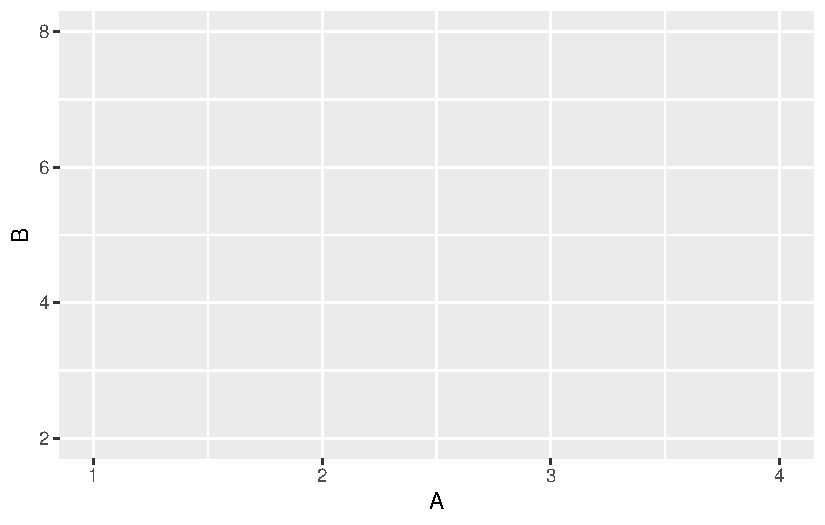
\includegraphics{Intro_to__ggplot_files/figure-pdf/unnamed-chunk-9-1.pdf}

}

\end{figure}

We can see that the aesthetic layer now applied to the plot scales the
data to present \texttt{A} along the x-axis with a range from lowest to
highest value from that vector. Similarly, the mapping presents
\texttt{B} along the y-axis with a range from lowest to highest value in
the vector. Also, the aesthetics include the variable name as a the
label for the x and y axes. Of course, these could be changed in a layer
as well. More on that later.

You might have been tempted to pass the variable names a quoted strings
(e.g., ``A'' and ``B) but if you do that, you'll get something
different.

\begin{Shaded}
\begin{Highlighting}[]
\FunctionTok{ggplot}\NormalTok{(}\AttributeTok{data =}\NormalTok{ DATA, }
       \AttributeTok{mapping =} \FunctionTok{aes}\NormalTok{(}\AttributeTok{x =} \StringTok{"C"}\NormalTok{, }\AttributeTok{y =} \StringTok{"B"}\NormalTok{)}
\NormalTok{       )}
\end{Highlighting}
\end{Shaded}

\begin{figure}[H]

{\centering 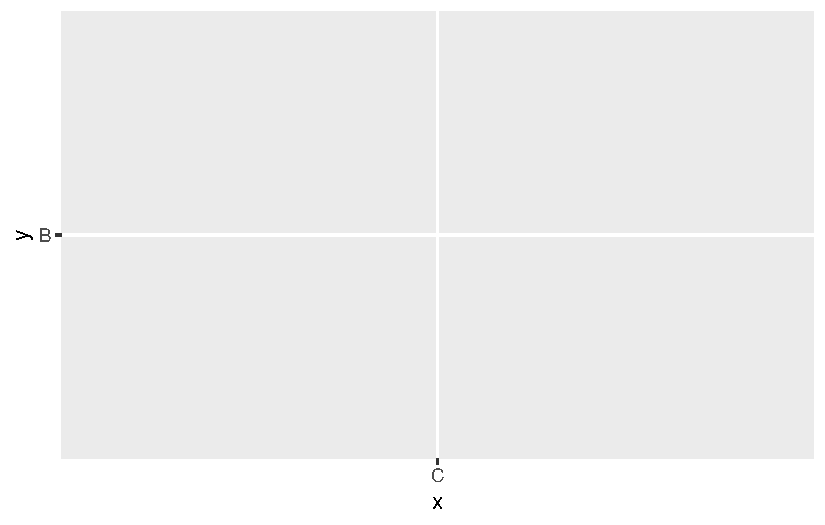
\includegraphics{Intro_to__ggplot_files/figure-pdf/unnamed-chunk-10-1.pdf}

}

\end{figure}

If we want to plot the data as they are in the data frame, we would
apply the `identity' transformation. By identity, we just need to
instruct \texttt{ggplot} to use the data values in the data set. If you
wanted to plot the means, frequency count, or something else, we would
need to tell \texttt{ggplot} how to transform the data.

\hypertarget{adding-plot-geometries}{%
\subsection{\texorpdfstring{\emph{Adding Plot
Geometries}}{Adding Plot Geometries}}\label{adding-plot-geometries}}

We don't yet have any geometries, or \emph{geoms}, added. Geoms can take
many forms, including, points, lines, bars, text, etc. If we want the
values in \texttt{A} and \texttt{B} to be plotted as x and y coordinates
representing points on the plot, we can add a point geometry using
\texttt{geom\_point()}.

\begin{Shaded}
\begin{Highlighting}[]
\FunctionTok{ggplot}\NormalTok{(}\AttributeTok{data =}\NormalTok{ DATA, }
       \AttributeTok{mapping =} \FunctionTok{aes}\NormalTok{(}\AttributeTok{x =}\NormalTok{ A, }\AttributeTok{y =}\NormalTok{ B)}
\NormalTok{       ) }\SpecialCharTok{+}
  \FunctionTok{geom\_point}\NormalTok{()}
\end{Highlighting}
\end{Shaded}

\begin{figure}[H]

{\centering 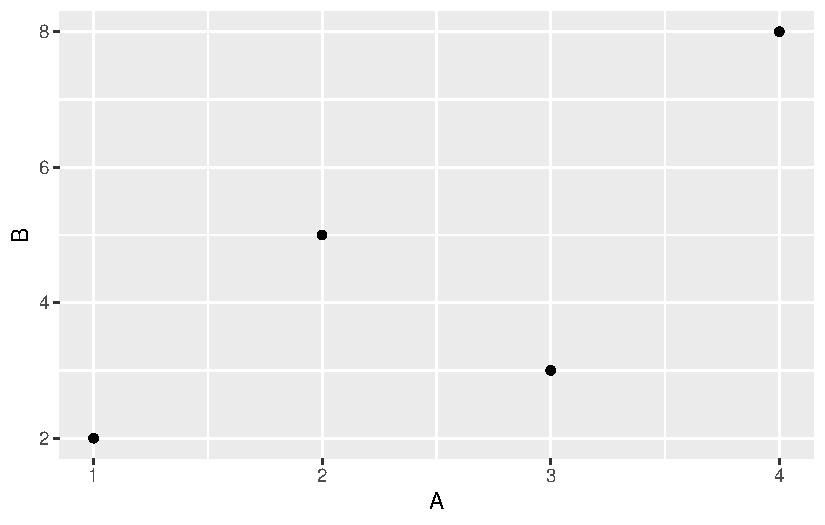
\includegraphics{Intro_to__ggplot_files/figure-pdf/unnamed-chunk-11-1.pdf}

}

\end{figure}

The points geometry has now been applied, which takes the aesthetic
mapping and makes them into points.

But geometries also have aesthetics, or visual properties so for each
geom, you can pass arguments to \texttt{aes()}. For example, the xy
points have to take some shape, color, and size in order for them to be
visible. By default, these have been determined or otherwise you
wouldn't see black circles of any size.

Checking \texttt{?geom\_point}, you will see at the bottom of the
arguments section, that by default \texttt{inherit.aes\ =\ TRUE}, which
means the aesthetic mappings in \texttt{geom\_point()} will be inherited
by default. Similarly, \texttt{data\ =\ NULL} so the data and the
aesthetic mapping from \texttt{ggplot()} don't need to be specified as
\texttt{data\ =\ DATA} and \texttt{mapping\ =\ aes(x\ =\ A,\ y\ =\ B)},
unless of course we wanted to overwrite them. Though not inherited,
other aesthetics have defaults for \texttt{geom\_point()}. If we wanted
to be verbose, we could include all of them and see how this plot
compares with that above.

\begin{Shaded}
\begin{Highlighting}[]
\FunctionTok{ggplot}\NormalTok{(}\AttributeTok{data =}\NormalTok{ DATA, }
       \AttributeTok{mapping =} \FunctionTok{aes}\NormalTok{(}\AttributeTok{x =}\NormalTok{ A, }\AttributeTok{y =}\NormalTok{ B)}
\NormalTok{       ) }\SpecialCharTok{+}
  \FunctionTok{geom\_point}\NormalTok{(}\AttributeTok{mapping =} \FunctionTok{aes}\NormalTok{(}\AttributeTok{x =}\NormalTok{ A, }\AttributeTok{y =}\NormalTok{ B),   }
             \AttributeTok{data =} \ConstantTok{NULL}\NormalTok{, }
             \AttributeTok{stat =} \StringTok{"identity"}\NormalTok{, }
             \AttributeTok{position =} \StringTok{"identity"}\NormalTok{, }
             \AttributeTok{size =} \FloatTok{1.5}\NormalTok{)}
\end{Highlighting}
\end{Shaded}

\begin{figure}[H]

{\centering 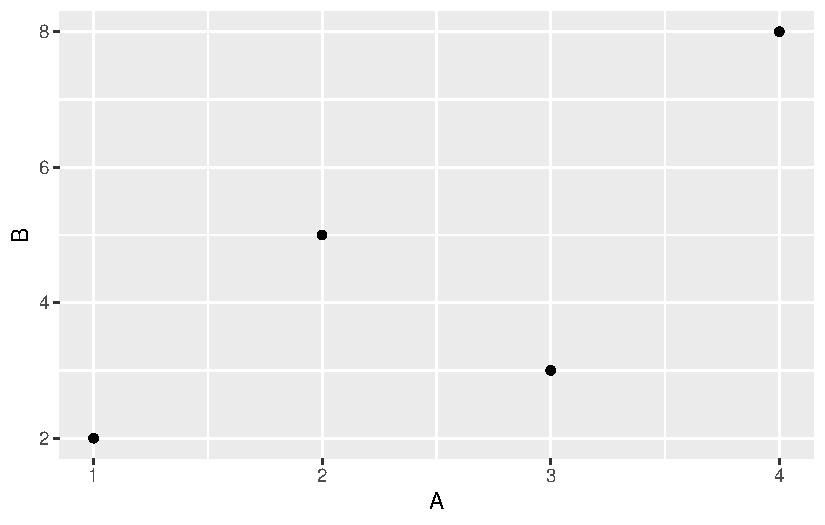
\includegraphics{Intro_to__ggplot_files/figure-pdf/unnamed-chunk-12-1.pdf}

}

\end{figure}

\hypertarget{how-and-where-to-map-aesthetics}{%
\subsubsection{\texorpdfstring{\emph{How and Where to Map
Aesthetics?}}{How and Where to Map Aesthetics?}}\label{how-and-where-to-map-aesthetics}}

You might be wondering how you map these aesthetic properties so that
when you attempt to do so, you don't get a bunch of errors. There are
two places you can map aesthetics:

Either in the initialized plot object:

\begin{itemize}
\tightlist
\item
  \textbf{\texttt{ggplot(data\ =\ data,\ mapping\ =\ aes(x,\ y))}}
  \texttt{+\ geom\_point()}
\end{itemize}

Or in the geometry:

\begin{itemize}
\tightlist
\item
  \texttt{ggplot()\ +}\textbf{\texttt{geom\_point(data\ =\ data,\ mapping\ =\ aes(x,\ y))}}
\end{itemize}

We can map aesthetics in the initialize plot object by also assigning
this to an object named \texttt{map} just so we can reference it as
need. When we do this mapping\ldots{}

\begin{Shaded}
\begin{Highlighting}[]
\NormalTok{map }\OtherTok{\textless{}{-}} \FunctionTok{ggplot}\NormalTok{(}\AttributeTok{data =}\NormalTok{ DATA, }
              \AttributeTok{mapping =} \FunctionTok{aes}\NormalTok{(A, C))}
\end{Highlighting}
\end{Shaded}

The aesthetics are inherited by the geometries that follow, which then
do not require any mapping of their own\ldots{}

\begin{Shaded}
\begin{Highlighting}[]
\NormalTok{map }\SpecialCharTok{+} 
  \FunctionTok{geom\_point}\NormalTok{() }\SpecialCharTok{+} 
  \FunctionTok{geom\_line}\NormalTok{()}
\end{Highlighting}
\end{Shaded}

\begin{figure}[H]

{\centering 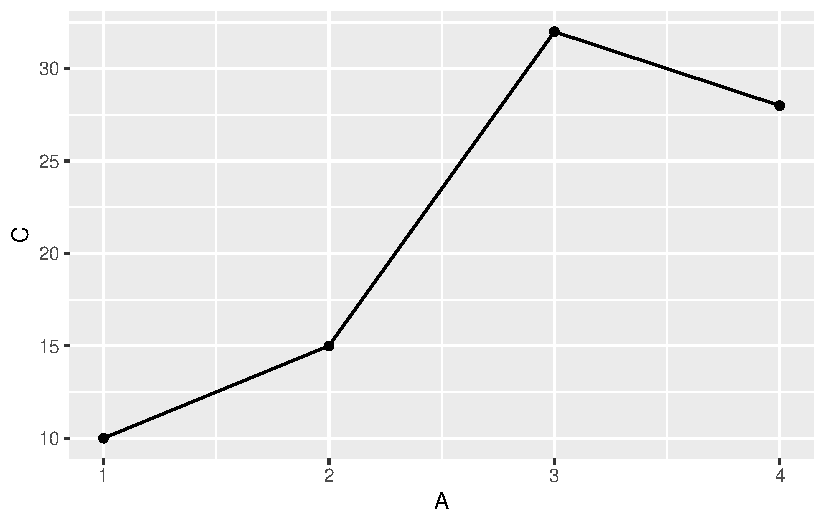
\includegraphics{Intro_to__ggplot_files/figure-pdf/unnamed-chunk-14-1.pdf}

}

\end{figure}

But when aesthetics are NOT mapped in initialized plot\ldots{}

\begin{Shaded}
\begin{Highlighting}[]
\NormalTok{map }\OtherTok{\textless{}{-}} \FunctionTok{ggplot}\NormalTok{() }
\end{Highlighting}
\end{Shaded}

There are no aesthetics to be inherited by the plot geometry functions
because they are not passed to the \texttt{ggplot()} object. In this
case they must be mapped as arguments the geometries themselves.

Plot points\ldots{}

\begin{Shaded}
\begin{Highlighting}[]
\NormalTok{map }\SpecialCharTok{+} 
  \FunctionTok{geom\_point}\NormalTok{(}\AttributeTok{data =}\NormalTok{ DATA, }
             \AttributeTok{mapping =} \FunctionTok{aes}\NormalTok{(A, C)) }
\end{Highlighting}
\end{Shaded}

\begin{figure}[H]

{\centering 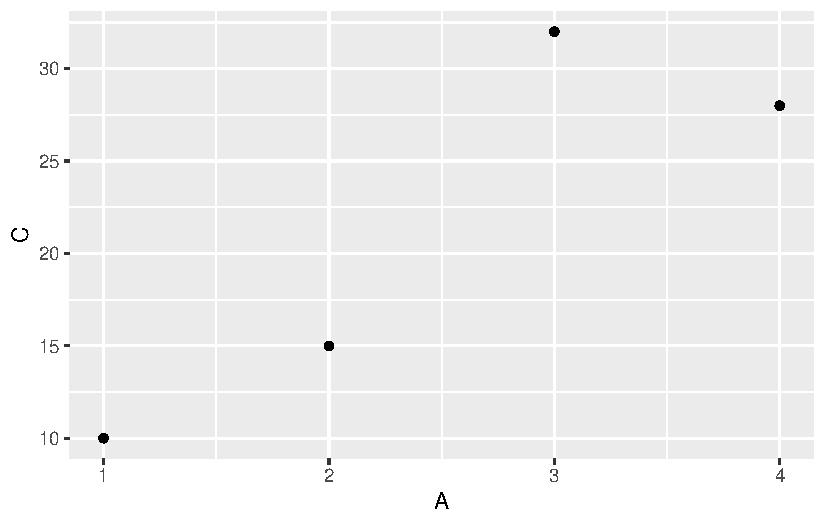
\includegraphics{Intro_to__ggplot_files/figure-pdf/unnamed-chunk-16-1.pdf}

}

\end{figure}

Plot a line\ldots{}

\begin{Shaded}
\begin{Highlighting}[]
\NormalTok{map }\SpecialCharTok{+} 
  \FunctionTok{geom\_line}\NormalTok{(}\AttributeTok{data =}\NormalTok{ DATA, }
            \AttributeTok{mapping =} \FunctionTok{aes}\NormalTok{(}\AttributeTok{x =}\NormalTok{ A, }\AttributeTok{y =}\NormalTok{ B))}
\end{Highlighting}
\end{Shaded}

\begin{figure}[H]

{\centering 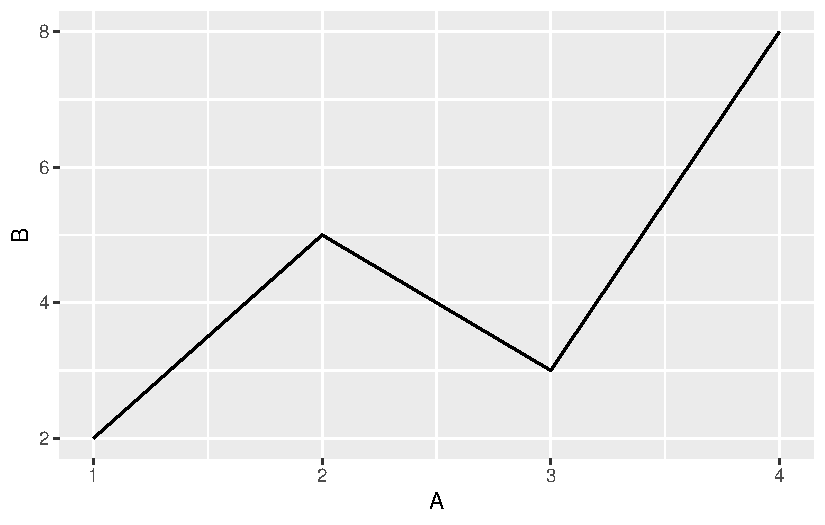
\includegraphics{Intro_to__ggplot_files/figure-pdf/unnamed-chunk-17-1.pdf}

}

\end{figure}

In a later section, we will differentiate between setting and mapping
aesthetic attributes.

\emph{Add labels, a coordinate system, scaling, and a theme}

Pretty much the same? For completeness, there are also x and y label
layers and a coordinate system also applied by default. Let's add them
to the plot by adding layers.

\begin{Shaded}
\begin{Highlighting}[]
\FunctionTok{ggplot}\NormalTok{(}\AttributeTok{data =}\NormalTok{ DATA, }
       \AttributeTok{mapping =} \FunctionTok{aes}\NormalTok{(}\AttributeTok{x =}\NormalTok{ A, }\AttributeTok{y =}\NormalTok{ B)}
\NormalTok{       ) }\SpecialCharTok{+}
  \FunctionTok{geom\_point}\NormalTok{(}\AttributeTok{mapping =} \FunctionTok{aes}\NormalTok{(}\AttributeTok{x =}\NormalTok{ A, }\AttributeTok{y =}\NormalTok{ B),   }
             \AttributeTok{data =} \ConstantTok{NULL}\NormalTok{, }
             \AttributeTok{stat =} \StringTok{"identity"}\NormalTok{, }
             \AttributeTok{position =} \StringTok{"identity"}\NormalTok{, }
             \AttributeTok{size =} \FloatTok{1.5}\NormalTok{,}
             \AttributeTok{color =} \StringTok{"black"}\NormalTok{) }\SpecialCharTok{+}
  \FunctionTok{scale\_x\_continuous}\NormalTok{() }\SpecialCharTok{+}
  \FunctionTok{scale\_y\_continuous}\NormalTok{() }\SpecialCharTok{+}
  \FunctionTok{labs}\NormalTok{(}\AttributeTok{title =} \StringTok{""}\NormalTok{) }\SpecialCharTok{+}
  \FunctionTok{xlab}\NormalTok{(}\StringTok{"A"}\NormalTok{) }\SpecialCharTok{+}
  \FunctionTok{ylab}\NormalTok{(}\StringTok{"B"}\NormalTok{) }\SpecialCharTok{+}
  \FunctionTok{coord\_cartesian}\NormalTok{() }\SpecialCharTok{+}
  \FunctionTok{theme}\NormalTok{()}
\end{Highlighting}
\end{Shaded}

\begin{figure}[H]

{\centering 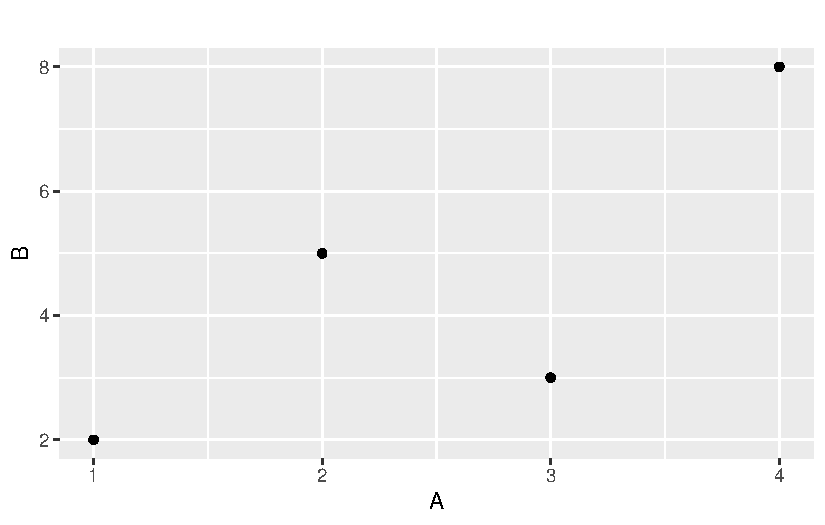
\includegraphics{Intro_to__ggplot_files/figure-pdf/unnamed-chunk-18-1.pdf}

}

\end{figure}

Notice the plot is the same. The take-home message is that each
visualization uses a data set which will be used to provide some
aesthetic mapping. That mapping takes some geometric form, or geom. The
geom needs information about the data, the statistical transformation
(or an its `identity' in the data frame), some position in space, some
size, and some color. Also the axes have labels and follow some rules
about their scaling. All of this follows some coordinate system. A theme
is also used to decorate the plot in different ways. The default is
\texttt{theme()}.

\emph{Change the coordinate system, color, and labels}

If we wanted to change the coordinate system, then the visualization
would look much different. We can also change the color and label names.
And because they are independent layers, we could add them in different
orders.

\begin{Shaded}
\begin{Highlighting}[]
\FunctionTok{ggplot}\NormalTok{(}\AttributeTok{data =}\NormalTok{ DATA, }
       \AttributeTok{mapping =} \FunctionTok{aes}\NormalTok{(}\AttributeTok{x =}\NormalTok{ A, }\AttributeTok{y =}\NormalTok{ B)}
\NormalTok{       ) }\SpecialCharTok{+}
  \FunctionTok{geom\_point}\NormalTok{(}\AttributeTok{mapping =} \FunctionTok{aes}\NormalTok{(}\AttributeTok{x =}\NormalTok{ A, }\AttributeTok{y =}\NormalTok{ B),   }
             \AttributeTok{data =} \ConstantTok{NULL}\NormalTok{, }
             \AttributeTok{stat =} \StringTok{"identity"}\NormalTok{, }
             \AttributeTok{position =} \StringTok{"identity"}\NormalTok{, }
             \AttributeTok{size =} \FloatTok{1.5}\NormalTok{,}
             \AttributeTok{color =} \StringTok{"blue"}\NormalTok{) }\SpecialCharTok{+}
  \FunctionTok{coord\_polar}\NormalTok{() }\SpecialCharTok{+}
  \FunctionTok{xlab}\NormalTok{(}\StringTok{"A Variable"}\NormalTok{) }\SpecialCharTok{+}
  \FunctionTok{ylab}\NormalTok{(}\StringTok{"B Variable"}\NormalTok{) }\SpecialCharTok{+}
  \FunctionTok{scale\_x\_continuous}\NormalTok{() }\SpecialCharTok{+}
  \FunctionTok{scale\_y\_continuous}\NormalTok{() }\SpecialCharTok{+}
  \FunctionTok{theme\_minimal}\NormalTok{()}
\end{Highlighting}
\end{Shaded}

\begin{figure}[H]

{\centering 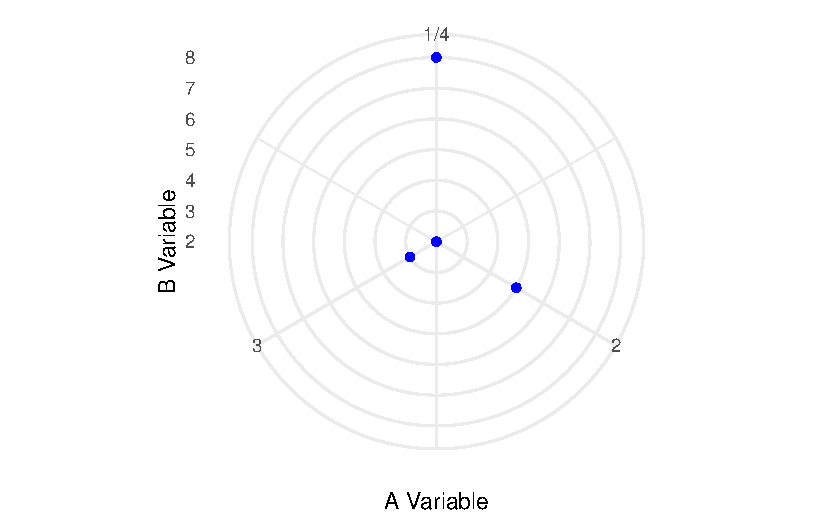
\includegraphics{Intro_to__ggplot_files/figure-pdf/unnamed-chunk-19-1.pdf}

}

\end{figure}

But because those are defaults, we don't need to code all those plot
layers. We can simply add a \texttt{geom\_point()} layer. And because we
pass \texttt{DATA} as the first argument and the mapping next, we could
be even less wordy.

\begin{Shaded}
\begin{Highlighting}[]
\FunctionTok{ggplot}\NormalTok{(DATA, }\FunctionTok{aes}\NormalTok{(}\AttributeTok{x =}\NormalTok{ A, }\AttributeTok{y =}\NormalTok{ B)) }\SpecialCharTok{+}
  \FunctionTok{geom\_point}\NormalTok{()}
\end{Highlighting}
\end{Shaded}

\begin{figure}[H]

{\centering 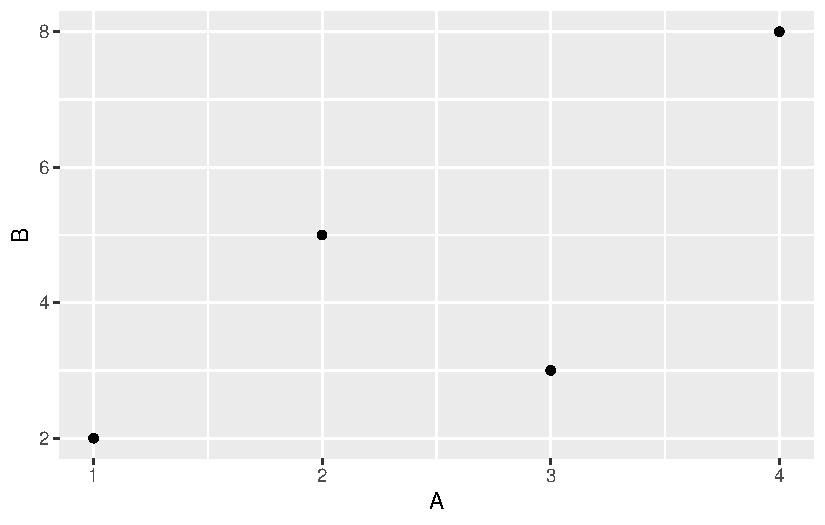
\includegraphics{Intro_to__ggplot_files/figure-pdf/unnamed-chunk-20-1.pdf}

}

\end{figure}

\hypertarget{some-geometries-and-their-aesthetics}{%
\section{\texorpdfstring{\textbf{Some Geometries and Their
Aesthetics}}{Some Geometries and Their Aesthetics}}\label{some-geometries-and-their-aesthetics}}

Not all geometries are the same. Although many geoms share most
aesthetics, they don't all have the same aesthetics. For example, a
point plot doesn't have aesthetics for a line but a line plot does. You
can only add aesthetics to geoms that are understood; adding those that
are not understood will, of course, throw errors.

\texttt{geom\_point()} understands these aesthetics:

\begin{itemize}
\tightlist
\item
  x
\item
  y
\item
  alpha
\item
  color
\item
  fill
\item
  group
\item
  shape
\item
  size
\item
  stroke
\end{itemize}

\texttt{geom\_line()} understands these aesthetics:

\begin{itemize}
\tightlist
\item
  x
\item
  y
\item
  alpha
\item
  color
\item
  fill
\item
  group
\item
  linetype
\item
  size
\end{itemize}

\texttt{geom\_bar()} understands these aesthetics:

\begin{itemize}
\tightlist
\item
  x
\item
  y
\item
  alpha
\item
  color
\item
  group
\item
  linetype
\item
  size
\end{itemize}

\texttt{geom\_col()} understands these aesthetics:

\begin{itemize}
\tightlist
\item
  x
\item
  y
\item
  alpha
\item
  color
\item
  fill
\item
  group
\item
  linetype
\item
  size
\end{itemize}

\hypertarget{adding-aesthetics-that-a-geometry-does-not-understand}{%
\section{\texorpdfstring{\textbf{Adding Aesthetics That A Geometry Does
not
Understand}}{Adding Aesthetics That A Geometry Does not Understand}}\label{adding-aesthetics-that-a-geometry-does-not-understand}}

If an aesthetic is not understood by a certain geometry, we cannot pass
are argument for it. For example, you cannot add a linetype to a point
plot. If you want your points connected by lines, then you can add a new
geom layer to the plot that contains that aesthetic. Importantly,
because geoms will inherit the data and mapping from \texttt{ggplot()}
by default, the line will connect the points.

\begin{Shaded}
\begin{Highlighting}[]
\FunctionTok{ggplot}\NormalTok{(DATA, }\FunctionTok{aes}\NormalTok{(}\AttributeTok{x =}\NormalTok{ A, }\AttributeTok{y =}\NormalTok{ B)) }\SpecialCharTok{+}
  \FunctionTok{geom\_point}\NormalTok{() }\SpecialCharTok{+}
  \FunctionTok{geom\_line}\NormalTok{()}
\end{Highlighting}
\end{Shaded}

\begin{figure}[H]

{\centering 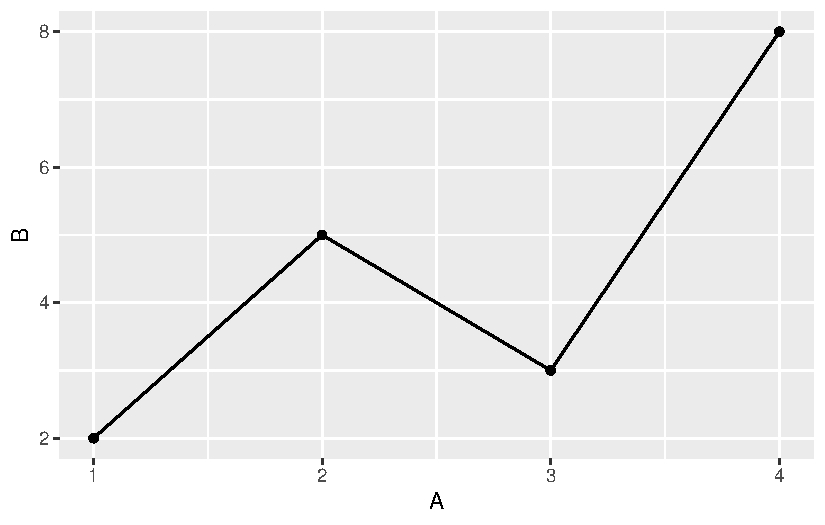
\includegraphics{Intro_to__ggplot_files/figure-pdf/unnamed-chunk-21-1.pdf}

}

\end{figure}

And then you can change the aesthetics of \texttt{geom\_line()} that it
understands. More one this later.

\hypertarget{aesthetic-mapping-versus-setting}{%
\section{\texorpdfstring{\textbf{Aesthetic Mapping Versus
Setting}}{Aesthetic Mapping Versus Setting}}\label{aesthetic-mapping-versus-setting}}

When adding aesthetics to a geom, you may wish to make an aesthetic
property like color a particular color such that all points in the point
plot are the same color or you may wish the point color to vary in some
way across the observations of the variable (e.g., change from cold to
hot color depending on the value). Similarly, you may wish to vary the
shape property with the value. You may even with the property to vary
corresponding to a different variable.

\begin{itemize}
\tightlist
\item
  \emph{setting} an aesthetic to a constant
\item
  \emph{mapping} an aesthetic to a variable
\end{itemize}

The difference between mapping and setting aesthetics all takes place
either in the \texttt{aes()} function or outside the functions of the
geometry. Because geometries understand certain aesthetics, the geom
function has a parameter for which you can pass an argument.

Because \texttt{geom\_point()} understands a \texttt{size} aesthetic
because points have to take some size. The default value for size is
assumed and passed in the first code block (you just don't see it) and
\texttt{size\ =\ 4} in the second code block overrides that default.

\begin{Shaded}
\begin{Highlighting}[]
\FunctionTok{ggplot}\NormalTok{(}\AttributeTok{data =}\NormalTok{ DATA, }\FunctionTok{aes}\NormalTok{(}\AttributeTok{x =}\NormalTok{ A, }\AttributeTok{y =}\NormalTok{ B)) }\SpecialCharTok{+} 
  \FunctionTok{geom\_point}\NormalTok{()}
\end{Highlighting}
\end{Shaded}

\begin{figure}[H]

{\centering 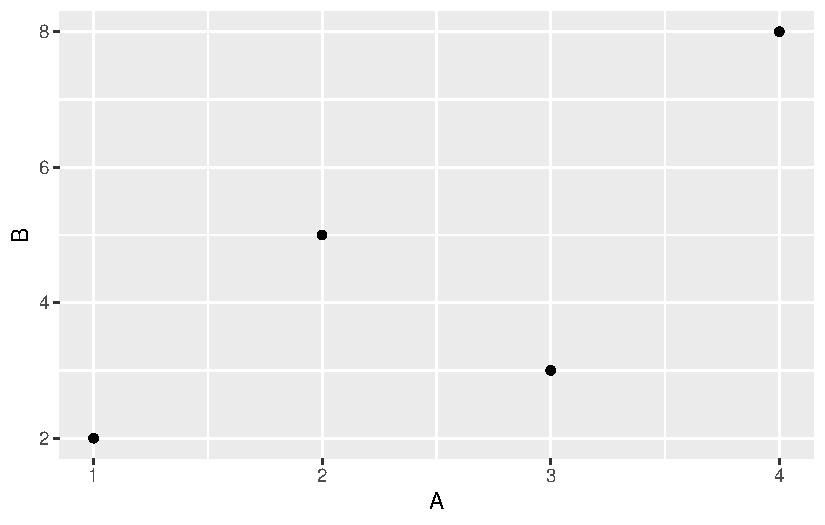
\includegraphics{Intro_to__ggplot_files/figure-pdf/unnamed-chunk-22-1.pdf}

}

\end{figure}

\begin{Shaded}
\begin{Highlighting}[]
\FunctionTok{ggplot}\NormalTok{(}\AttributeTok{data =}\NormalTok{ DATA, }\FunctionTok{aes}\NormalTok{(}\AttributeTok{x =}\NormalTok{ A, }\AttributeTok{y =}\NormalTok{ B)) }\SpecialCharTok{+} 
  \FunctionTok{geom\_point}\NormalTok{(}\AttributeTok{size =} \DecValTok{4}\NormalTok{)}
\end{Highlighting}
\end{Shaded}

\begin{figure}[H]

{\centering 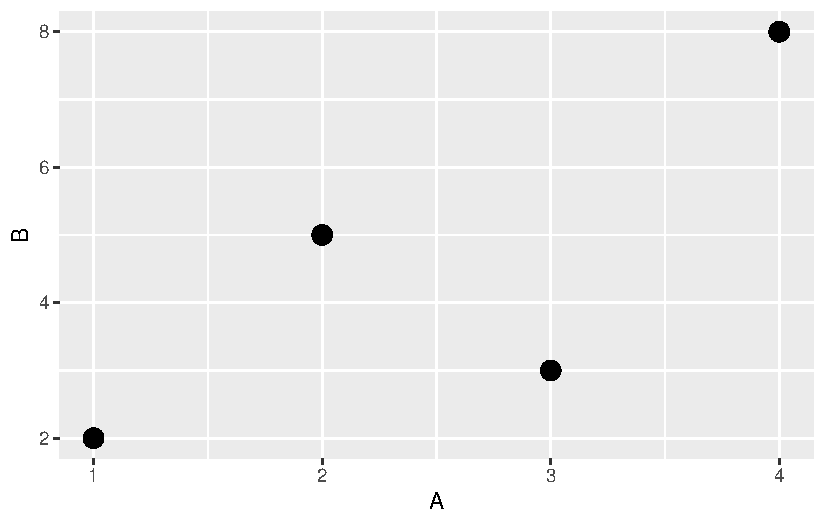
\includegraphics{Intro_to__ggplot_files/figure-pdf/unnamed-chunk-22-2.pdf}

}

\end{figure}

By passing \texttt{size\ =\ 4}, we have \emph{set} size to a
\emph{constant} value. Not that at size was not passed inside an
\texttt{aes()} function. It it were, something completely different
would happen.

\begin{Shaded}
\begin{Highlighting}[]
\FunctionTok{ggplot}\NormalTok{(}\AttributeTok{data =}\NormalTok{ DATA, }\FunctionTok{aes}\NormalTok{(}\AttributeTok{x =}\NormalTok{ A, }\AttributeTok{y =}\NormalTok{ B)) }\SpecialCharTok{+} 
  \FunctionTok{geom\_point}\NormalTok{(}\FunctionTok{aes}\NormalTok{(}\AttributeTok{size =} \DecValTok{7}\NormalTok{))}
\end{Highlighting}
\end{Shaded}

\begin{figure}[H]

{\centering 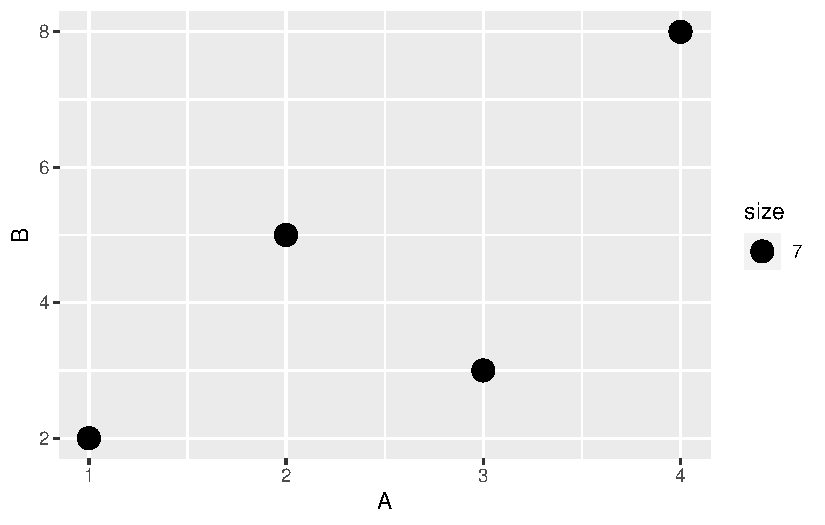
\includegraphics{Intro_to__ggplot_files/figure-pdf/unnamed-chunk-23-1.pdf}

}

\end{figure}

And this is illustrated even better with the \texttt{color} aesthetic.

\begin{Shaded}
\begin{Highlighting}[]
\FunctionTok{ggplot}\NormalTok{(}\AttributeTok{data =}\NormalTok{ DATA, }\FunctionTok{aes}\NormalTok{(}\AttributeTok{x =}\NormalTok{ A, }\AttributeTok{y =}\NormalTok{ B)) }\SpecialCharTok{+} 
  \FunctionTok{geom\_point}\NormalTok{(}\FunctionTok{aes}\NormalTok{(}\AttributeTok{color =} \StringTok{"blue"}\NormalTok{))}
\end{Highlighting}
\end{Shaded}

\begin{figure}[H]

{\centering 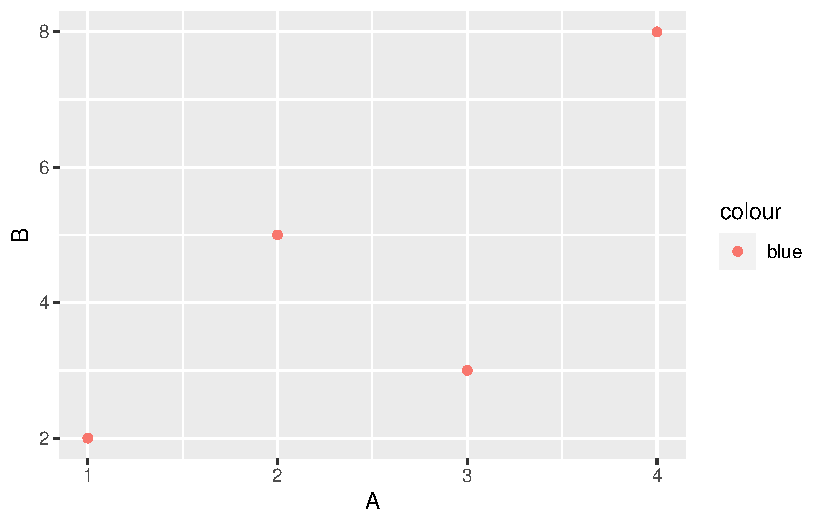
\includegraphics{Intro_to__ggplot_files/figure-pdf/unnamed-chunk-24-1.pdf}

}

\end{figure}

In both examples, you notice that a legend not appears in the plot and
in the color example, the color is not blue. Without getting into the
details of what ggplot is doing, when this happens, it serves as a
warning that you did something incorrectly.

Importantly, you can only \emph{set constant values} to aesthetics
outside of \texttt{aes()}. Inside of \texttt{aes()}, you \emph{map
variables} to aesthetics. Where are the variables? Well, in the data
frame. By passing a different variable column form \texttt{DATA}, we can
\emph{map} the aesthetic to that \emph{variable} so that it changes
relative to the changes in the variable. The plot will also change in a
variety of ways simply by adding a new variable. Let's begin with a
baseline plot for comparison and then map variables.

\begin{Shaded}
\begin{Highlighting}[]
\FunctionTok{ggplot}\NormalTok{(}\AttributeTok{data =}\NormalTok{ DATA, }\FunctionTok{aes}\NormalTok{(}\AttributeTok{x =}\NormalTok{ A, }\AttributeTok{y =}\NormalTok{ B)) }\SpecialCharTok{+} 
  \FunctionTok{geom\_point}\NormalTok{()}
\end{Highlighting}
\end{Shaded}

\begin{figure}[H]

{\centering 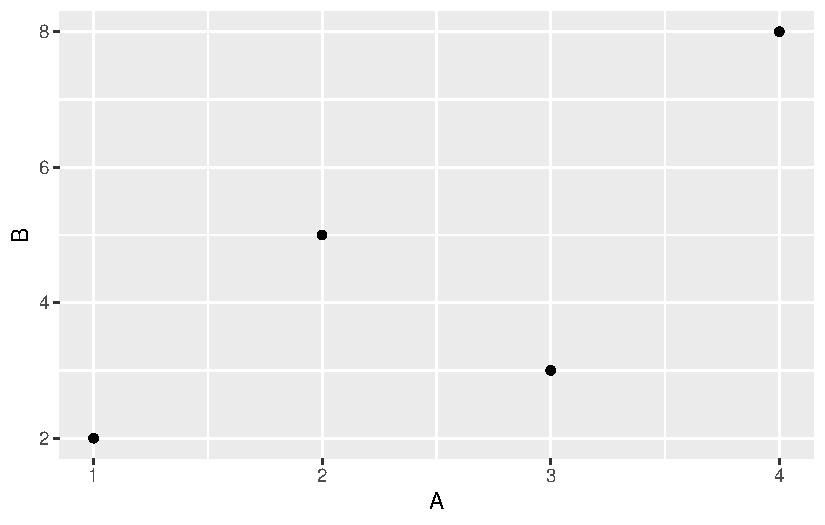
\includegraphics{Intro_to__ggplot_files/figure-pdf/unnamed-chunk-25-1.pdf}

}

\end{figure}

\hypertarget{mapping-a-new-variable}{%
\subsection{\texorpdfstring{\emph{Mapping a new
variable\ldots{}}}{Mapping a new variable\ldots{}}}\label{mapping-a-new-variable}}

\begin{Shaded}
\begin{Highlighting}[]
\FunctionTok{ggplot}\NormalTok{(}\AttributeTok{data =}\NormalTok{ DATA, }\FunctionTok{aes}\NormalTok{(}\AttributeTok{x =}\NormalTok{ A, }\AttributeTok{y =}\NormalTok{ B)) }\SpecialCharTok{+} 
  \FunctionTok{geom\_point}\NormalTok{(}\FunctionTok{aes}\NormalTok{(}\AttributeTok{color =}\NormalTok{ D))}
\end{Highlighting}
\end{Shaded}

\begin{figure}[H]

{\centering 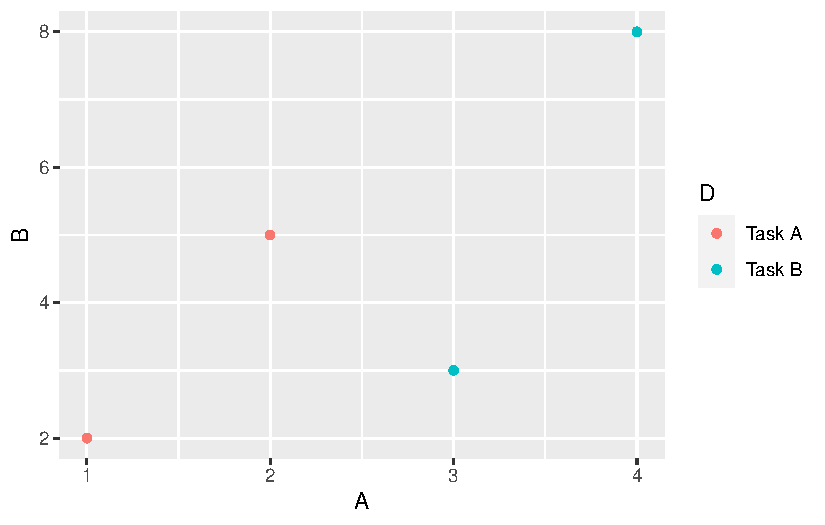
\includegraphics{Intro_to__ggplot_files/figure-pdf/unnamed-chunk-26-1.pdf}

}

\end{figure}

\hypertarget{mapping-an-existing-variable}{%
\subsection{\texorpdfstring{\emph{Mapping an existing
variable\ldots{}}}{Mapping an existing variable\ldots{}}}\label{mapping-an-existing-variable}}

\begin{Shaded}
\begin{Highlighting}[]
\FunctionTok{ggplot}\NormalTok{(}\AttributeTok{data =}\NormalTok{ DATA, }\FunctionTok{aes}\NormalTok{(}\AttributeTok{x =}\NormalTok{ A, }\AttributeTok{y =}\NormalTok{ B)) }\SpecialCharTok{+} 
  \FunctionTok{geom\_point}\NormalTok{(}\FunctionTok{aes}\NormalTok{(}\AttributeTok{color =}\NormalTok{ A))}
\end{Highlighting}
\end{Shaded}

\begin{figure}[H]

{\centering 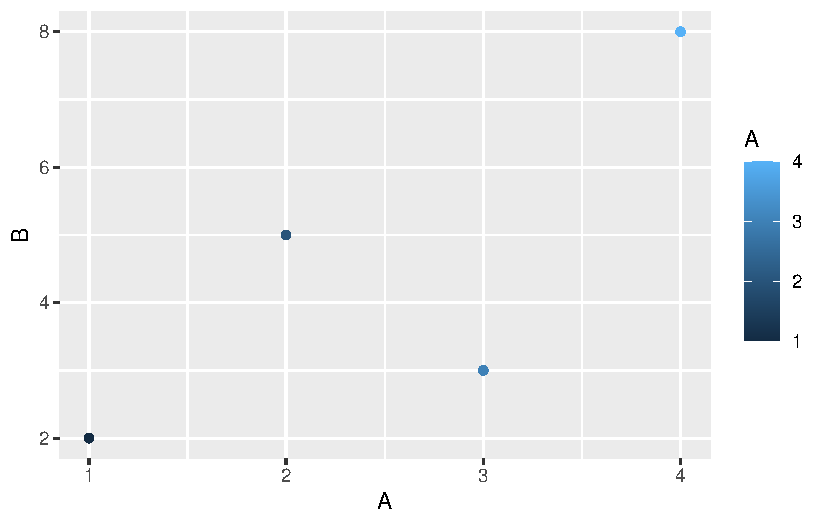
\includegraphics{Intro_to__ggplot_files/figure-pdf/unnamed-chunk-27-1.pdf}

}

\end{figure}

\begin{Shaded}
\begin{Highlighting}[]
\FunctionTok{ggplot}\NormalTok{(}\AttributeTok{data =}\NormalTok{ DATA, }\FunctionTok{aes}\NormalTok{(}\AttributeTok{x =}\NormalTok{ A, }\AttributeTok{y =}\NormalTok{ B)) }\SpecialCharTok{+} 
  \FunctionTok{geom\_point}\NormalTok{(}\FunctionTok{aes}\NormalTok{(}\AttributeTok{color =}\NormalTok{ B))}
\end{Highlighting}
\end{Shaded}

\begin{figure}[H]

{\centering 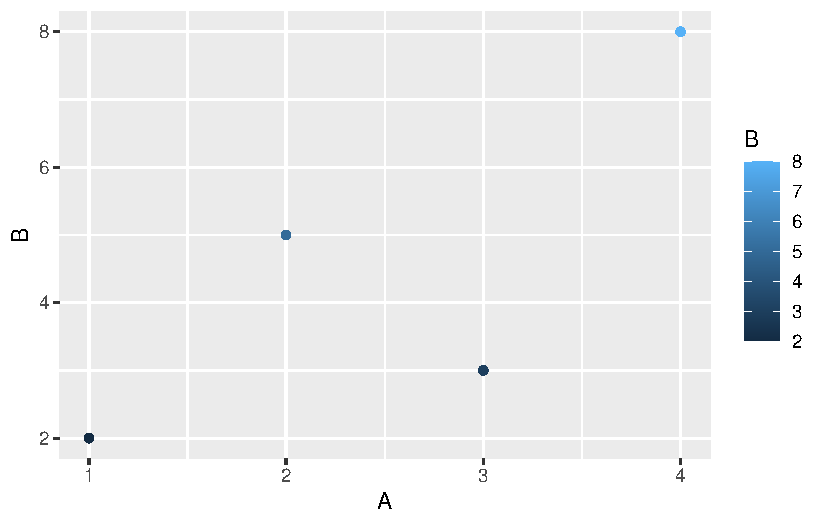
\includegraphics{Intro_to__ggplot_files/figure-pdf/unnamed-chunk-27-2.pdf}

}

\end{figure}

You may have noticed that when mapped variables are numeric, the
aesthetics are applied continuously and when they are categorical, they
are applied discretely. Here is a good example of mapping variable
\texttt{A} not as itself but by changing it to a \texttt{factor()} or a
character vector.

\begin{Shaded}
\begin{Highlighting}[]
\FunctionTok{ggplot}\NormalTok{(}\AttributeTok{data =}\NormalTok{ DATA, }\FunctionTok{aes}\NormalTok{(}\AttributeTok{x =}\NormalTok{ A, }\AttributeTok{y =}\NormalTok{ B)) }\SpecialCharTok{+} 
  \FunctionTok{geom\_point}\NormalTok{(}\FunctionTok{aes}\NormalTok{(}\AttributeTok{color =} \FunctionTok{as.factor}\NormalTok{(A)))}
\end{Highlighting}
\end{Shaded}

\begin{figure}[H]

{\centering 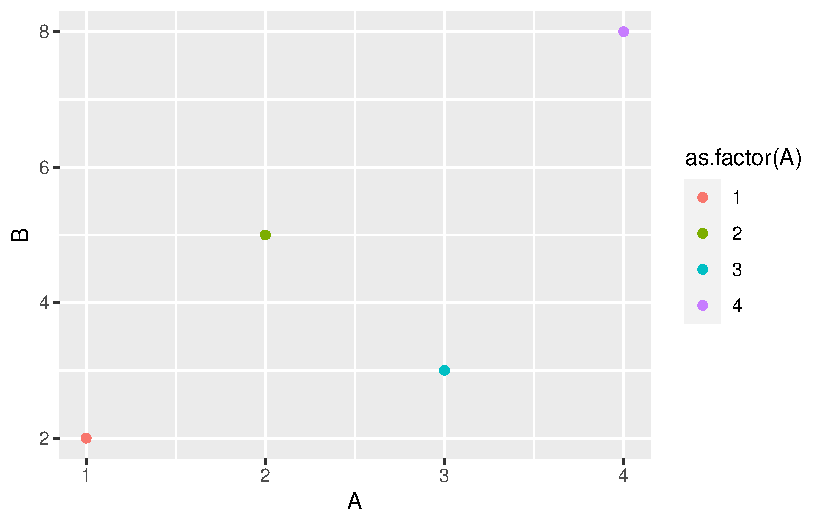
\includegraphics{Intro_to__ggplot_files/figure-pdf/unnamed-chunk-28-1.pdf}

}

\end{figure}

\begin{Shaded}
\begin{Highlighting}[]
\FunctionTok{ggplot}\NormalTok{(}\AttributeTok{data =}\NormalTok{ DATA, }\FunctionTok{aes}\NormalTok{(}\AttributeTok{x =}\NormalTok{ A, }\AttributeTok{y =}\NormalTok{ B)) }\SpecialCharTok{+} 
  \FunctionTok{geom\_point}\NormalTok{(}\FunctionTok{aes}\NormalTok{(}\AttributeTok{color =} \FunctionTok{as.character}\NormalTok{(A)))}
\end{Highlighting}
\end{Shaded}

\begin{figure}[H]

{\centering 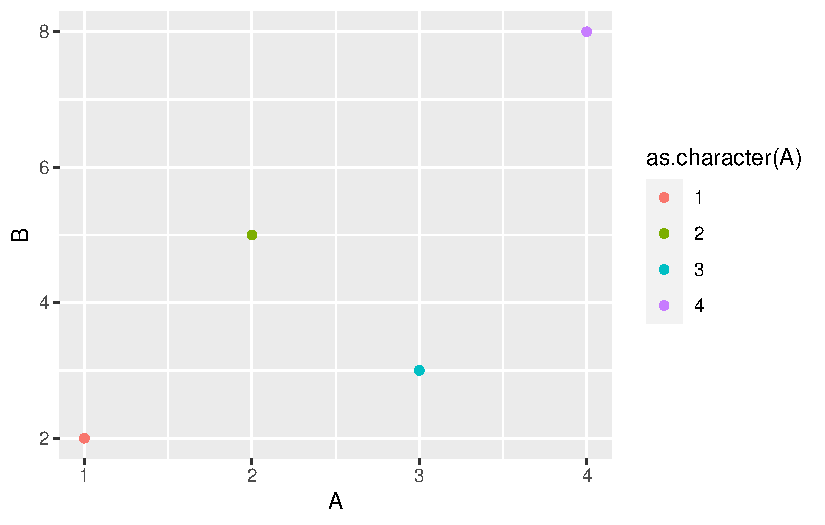
\includegraphics{Intro_to__ggplot_files/figure-pdf/unnamed-chunk-28-2.pdf}

}

\end{figure}

\hypertarget{setting-and-mapping-combinations}{%
\subsection{\texorpdfstring{\emph{Setting and Mapping
Combinations}}{Setting and Mapping Combinations}}\label{setting-and-mapping-combinations}}

We can also combine setting aesthetics and mapping them as long as
mappings are inside \texttt{aes()} and settings are not.

\begin{Shaded}
\begin{Highlighting}[]
\FunctionTok{ggplot}\NormalTok{(}\AttributeTok{data =}\NormalTok{ DATA, }\FunctionTok{aes}\NormalTok{(}\AttributeTok{x =}\NormalTok{ A, }\AttributeTok{y =}\NormalTok{ B)) }\SpecialCharTok{+} 
  \FunctionTok{geom\_point}\NormalTok{(}\AttributeTok{color =} \StringTok{"green"}\NormalTok{, }\FunctionTok{aes}\NormalTok{(}\AttributeTok{shape =}\NormalTok{ D))}
\end{Highlighting}
\end{Shaded}

\begin{figure}[H]

{\centering 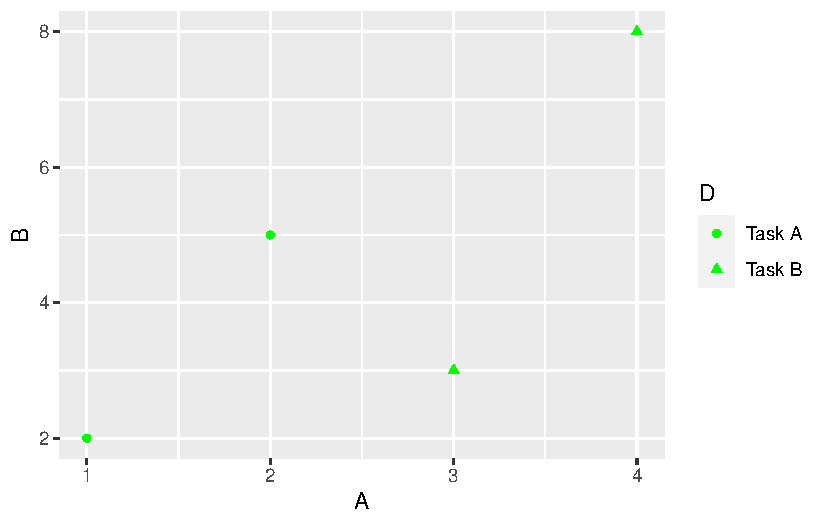
\includegraphics{Intro_to__ggplot_files/figure-pdf/unnamed-chunk-29-1.pdf}

}

\end{figure}

\begin{Shaded}
\begin{Highlighting}[]
\FunctionTok{ggplot}\NormalTok{(}\AttributeTok{data =}\NormalTok{ DATA, }\FunctionTok{aes}\NormalTok{(}\AttributeTok{x =}\NormalTok{ A, }\AttributeTok{y =}\NormalTok{ B)) }\SpecialCharTok{+} 
  \FunctionTok{geom\_point}\NormalTok{(}\AttributeTok{color =} \StringTok{"blue"}\NormalTok{, }\FunctionTok{aes}\NormalTok{(}\AttributeTok{size =}\NormalTok{ A))}
\end{Highlighting}
\end{Shaded}

\begin{figure}[H]

{\centering 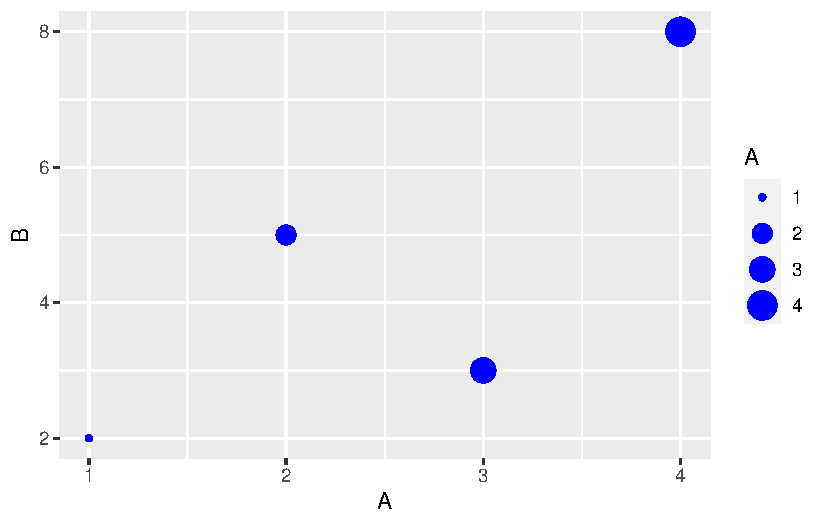
\includegraphics{Intro_to__ggplot_files/figure-pdf/unnamed-chunk-29-2.pdf}

}

\end{figure}

\begin{Shaded}
\begin{Highlighting}[]
\FunctionTok{ggplot}\NormalTok{(}\AttributeTok{data =}\NormalTok{ DATA, }\FunctionTok{aes}\NormalTok{(}\AttributeTok{x =}\NormalTok{ A, }\AttributeTok{y =}\NormalTok{ B)) }\SpecialCharTok{+} 
  \FunctionTok{geom\_point}\NormalTok{(}\AttributeTok{shape =} \DecValTok{21}\NormalTok{, }\FunctionTok{aes}\NormalTok{(}\AttributeTok{color =}\NormalTok{ D))}
\end{Highlighting}
\end{Shaded}

\begin{figure}[H]

{\centering 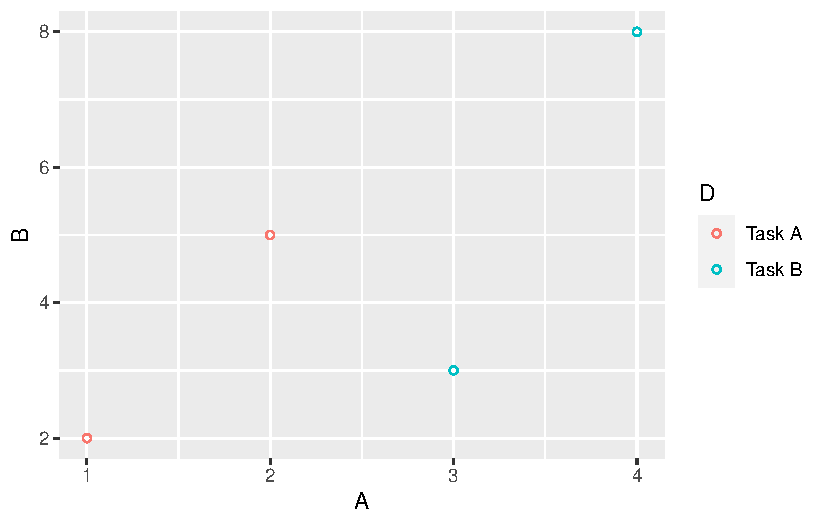
\includegraphics{Intro_to__ggplot_files/figure-pdf/unnamed-chunk-29-3.pdf}

}

\end{figure}

Importantly, just as you cannot pass constant values to aesthetics in
\texttt{aes()}, you cannot pass a variable to an aesthetic in the geom
function \emph{unless} it is inside \texttt{aes()}.

For example, passing \texttt{color\ =\ A} in this instance will throw an
error.

\texttt{ggplot(data\ =\ DATA,\ aes(x\ =\ A,\ y\ =\ B))\ +}
\texttt{geom\_point(color\ =\ A))}

\texttt{Error:\ unexpected\ \textquotesingle{})\textquotesingle{}\ in:}
\texttt{"ggplot(data\ =\ DATA,\ aes(x\ =\ A,\ y\ =\ B))\ +}
\texttt{geom\_point(color\ =\ A))"}

In summary, when you want to set an aesthetic to a constant value, do so
in the geometry function (e.g., \texttt{geom\_point()}), otherwise, pass
an \texttt{aes()} to the geometry function. Color options can be
discovered using \texttt{colors()}. Linetype has fewer options. To make
the color more or less transparent, adjust alpha (from 0 = invisible to
1).

\begin{Shaded}
\begin{Highlighting}[]
\FunctionTok{ggplot}\NormalTok{(DATA, }\FunctionTok{aes}\NormalTok{(}\AttributeTok{x =}\NormalTok{ A, }\AttributeTok{y =}\NormalTok{ B)) }\SpecialCharTok{+}
  \FunctionTok{geom\_point}\NormalTok{() }\SpecialCharTok{+}
  \FunctionTok{geom\_line}\NormalTok{(}\AttributeTok{linetype =} \StringTok{"dashed"}\NormalTok{,}
            \AttributeTok{color =} \StringTok{"red"}\NormalTok{,}
            \AttributeTok{alpha =}\NormalTok{ .}\DecValTok{3}\NormalTok{)}
\end{Highlighting}
\end{Shaded}

\begin{figure}[H]

{\centering 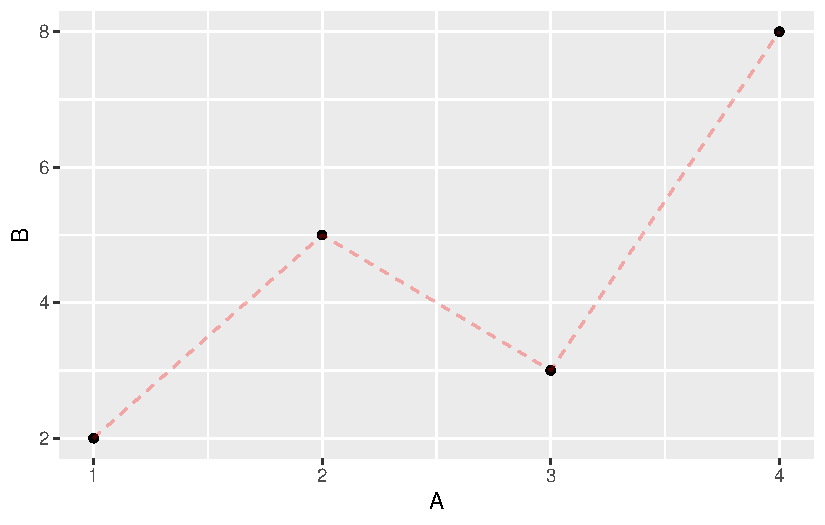
\includegraphics{Intro_to__ggplot_files/figure-pdf/unnamed-chunk-30-1.pdf}

}

\end{figure}

\hypertarget{histogram-and-density-chart-varieties}{%
\section{\texorpdfstring{\textbf{Histogram and Density Chart
Varieties}}{Histogram and Density Chart Varieties}}\label{histogram-and-density-chart-varieties}}

When you need to visualize the distribution of a single continuous
variable, a histogram is your friend. You may need to create bins (e.g.,
ranges) and count the number of observations in each bin. Thus,
histograms display the frequency counts with bars, so they will look
different based on binning. Similarly, frequency polygons, using
\texttt{geom\_freqpoly()} display the same information with lines. For
this example, we will use the \texttt{mtcars} data rather than the small
data frame \texttt{DATA}.

\hypertarget{geom_histogram}{%
\subsection{\texorpdfstring{\emph{\texttt{geom\_histogram()}}}{geom\_histogram()}}\label{geom_histogram}}

\begin{Shaded}
\begin{Highlighting}[]
\FunctionTok{ggplot}\NormalTok{(}\AttributeTok{data =}\NormalTok{ mtcars, }
       \AttributeTok{mapping =} \FunctionTok{aes}\NormalTok{(}\AttributeTok{x =}\NormalTok{ mpg)) }\SpecialCharTok{+}
  \FunctionTok{geom\_histogram}\NormalTok{()}
\end{Highlighting}
\end{Shaded}

\begin{verbatim}
`stat_bin()` using `bins = 30`. Pick better value with `binwidth`.
\end{verbatim}

\begin{figure}[H]

{\centering 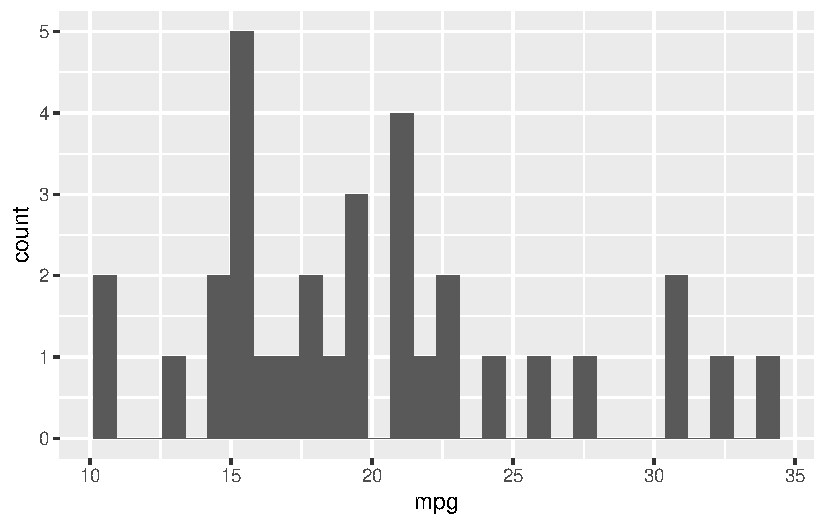
\includegraphics{Intro_to__ggplot_files/figure-pdf/unnamed-chunk-31-1.pdf}

}

\end{figure}

\begin{Shaded}
\begin{Highlighting}[]
\CommentTok{\# or less popular}
\FunctionTok{ggplot}\NormalTok{(}\AttributeTok{data =}\NormalTok{ mtcars, }
       \AttributeTok{mapping =} \FunctionTok{aes}\NormalTok{(}\AttributeTok{y =}\NormalTok{ mpg)) }\SpecialCharTok{+}
  \FunctionTok{geom\_histogram}\NormalTok{()}
\end{Highlighting}
\end{Shaded}

\begin{verbatim}
`stat_bin()` using `bins = 30`. Pick better value with `binwidth`.
\end{verbatim}

\begin{figure}[H]

{\centering 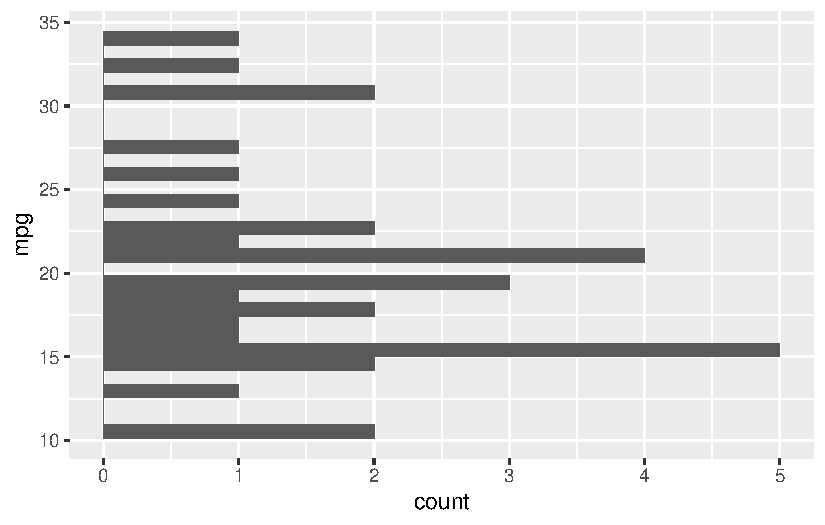
\includegraphics{Intro_to__ggplot_files/figure-pdf/unnamed-chunk-31-2.pdf}

}

\end{figure}

\hypertarget{geom_density}{%
\subsection{\texorpdfstring{\emph{\texttt{geom\_density()}}}{geom\_density()}}\label{geom_density}}

When you need a smoothed version of the histogram,
\texttt{geom\_density()} will produce a kernel density plot. In this
case, we also add \texttt{fill\ =\ cyl} to fill the densities by color.

\begin{Shaded}
\begin{Highlighting}[]
\FunctionTok{ggplot}\NormalTok{(}\AttributeTok{data =}\NormalTok{ mtcars, }
       \AttributeTok{mapping =} \FunctionTok{aes}\NormalTok{(}\AttributeTok{x =}\NormalTok{ mpg)) }\SpecialCharTok{+}
  \FunctionTok{geom\_density}\NormalTok{(}\AttributeTok{mapping =} \FunctionTok{aes}\NormalTok{(}\AttributeTok{fill =}\NormalTok{ cyl), }
               \AttributeTok{alpha =}\NormalTok{ .}\DecValTok{5}\NormalTok{)}
\end{Highlighting}
\end{Shaded}

\begin{verbatim}
Warning: The following aesthetics were dropped during statistical transformation: fill
i This can happen when ggplot fails to infer the correct grouping structure in
  the data.
i Did you forget to specify a `group` aesthetic or to convert a numerical
  variable into a factor?
\end{verbatim}

\begin{figure}[H]

{\centering 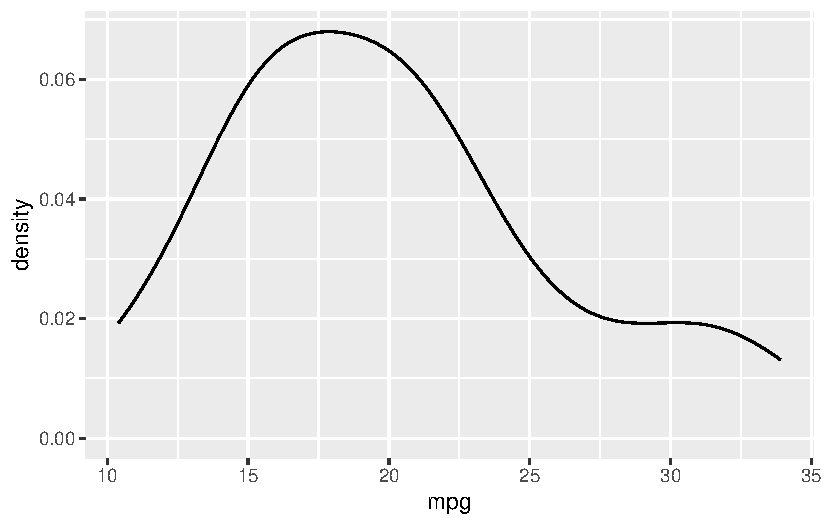
\includegraphics{Intro_to__ggplot_files/figure-pdf/unnamed-chunk-32-1.pdf}

}

\end{figure}

Wait, huh? But this does not fill the densities with a color
corresponding to \texttt{cyl}. Does it need to be a different type?

\begin{Shaded}
\begin{Highlighting}[]
\FunctionTok{ggplot}\NormalTok{(}\AttributeTok{data =}\NormalTok{ mtcars, }
       \AttributeTok{mapping =} \FunctionTok{aes}\NormalTok{(}\AttributeTok{x =}\NormalTok{ mpg)) }\SpecialCharTok{+}
  \FunctionTok{geom\_density}\NormalTok{(}\AttributeTok{mapping =} \FunctionTok{aes}\NormalTok{(}\AttributeTok{fill =} \FunctionTok{as.factor}\NormalTok{(cyl)),}
               \AttributeTok{alpha =}\NormalTok{ .}\DecValTok{5}\NormalTok{)}
\end{Highlighting}
\end{Shaded}

\begin{figure}[H]

{\centering 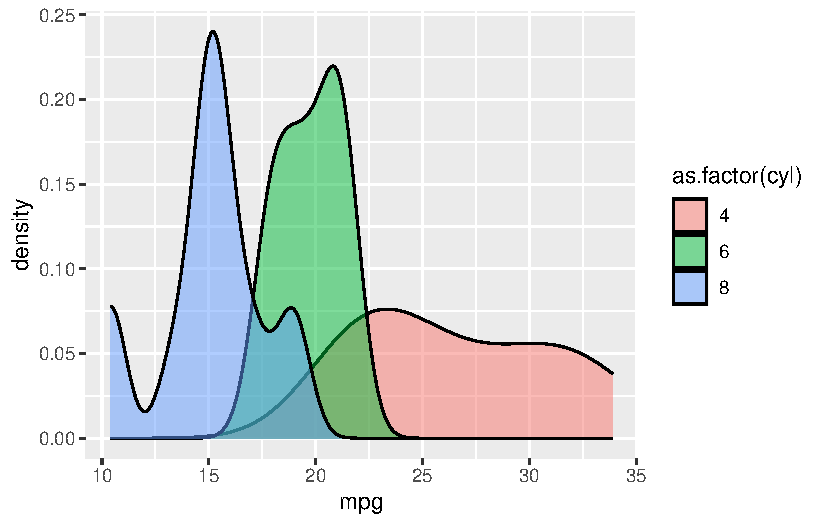
\includegraphics{Intro_to__ggplot_files/figure-pdf/unnamed-chunk-33-1.pdf}

}

\end{figure}

OK better, except for cleaning up the legend.

\hypertarget{bar-chart-varieties}{%
\section{\texorpdfstring{\textbf{Bar Chart
Varieties}}{Bar Chart Varieties}}\label{bar-chart-varieties}}

There are two types of bar chart geometry functions:
\texttt{geom\_bar()} and \texttt{geom\_col()}. \texttt{geom\_bar()}
takes either an \texttt{x} or a \texttt{y} (not both) and produces a
plot for which the height of the bar is proportional to the
count/frequency of cases in the vector. By contrast,
\texttt{geom\_col()} takes both an \texttt{x} and a \texttt{y} and plots
the height of each x variable bar relative to the value of the y
variable. If you want the heights of the bars to represent values in the
data, use \texttt{geom\_col()}

\hypertarget{geom_bar}{%
\subsection{\texorpdfstring{\emph{\texttt{geom\_bar()}}}{geom\_bar()}}\label{geom_bar}}

There are times you want bar plots.

Trying out \texttt{geom\_bar()}, we need an either an \texttt{x} or a
\texttt{y} aesthetic mapping but not both. When passing a variable to x,
the bar will be vertical and when passing the variable to y, the bar
will be horizontal. Because the mapping is inherited from
\texttt{ggplot()}, you'll throw an error like the following because both
x and y will be inherited:

\texttt{Error\ in\ f():}
\texttt{!\ stat\_count()\ can\ only\ have\ an\ x\ or\ y\ aesthetic.}

We can change the mapping in the base \texttt{ggplot()} layer, which
will plot bars corresponding to the unique levels of the variable passed
to \texttt{x} at a height relative to the frequency of occurrence of
those unique levels. To see what might be plotted from \texttt{A}, see
\texttt{DATA\$A} 1, 2, 3, 4.

Checking \texttt{?geom\_bar}, you will notice that \texttt{geom\_bar()}
has a default \texttt{stat\ =\ "count"}. This means that the default bar
plot will plot the \texttt{"count"}, or frequency of elements in a
vector variable. When the count or frequency of a value is 1, the bar
height will be 1 on the y axis and if an element appears 5 times in the
vector, the bar height will be 5. For a horizontal bar, the bar length,
rather than height, will be 5. Looking at \texttt{DATA\$A} 1, 2, 3, 4,
what might you expect the bar to look like?

\begin{Shaded}
\begin{Highlighting}[]
\CommentTok{\# setting x}
\NormalTok{DATA }\SpecialCharTok{\%\textgreater{}\%}
  \FunctionTok{ggplot}\NormalTok{(., }\FunctionTok{aes}\NormalTok{(}\AttributeTok{x =}\NormalTok{ A)) }\SpecialCharTok{+}
  \FunctionTok{geom\_bar}\NormalTok{()}
\end{Highlighting}
\end{Shaded}

\begin{figure}[H]

{\centering 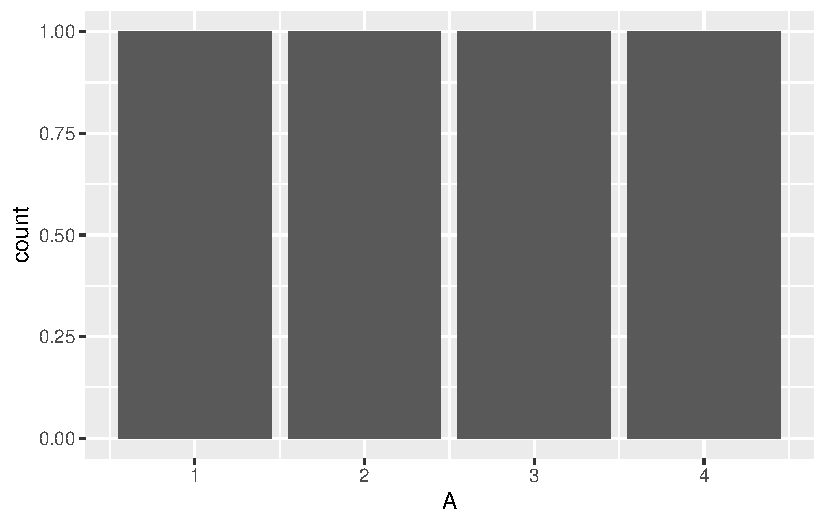
\includegraphics{Intro_to__ggplot_files/figure-pdf/unnamed-chunk-34-1.pdf}

}

\end{figure}

\begin{Shaded}
\begin{Highlighting}[]
\CommentTok{\# setting y}
\NormalTok{DATA }\SpecialCharTok{\%\textgreater{}\%}
  \FunctionTok{ggplot}\NormalTok{(., }\FunctionTok{aes}\NormalTok{(}\AttributeTok{y =}\NormalTok{ A)) }\SpecialCharTok{+}
  \FunctionTok{geom\_bar}\NormalTok{()}
\end{Highlighting}
\end{Shaded}

\begin{figure}[H]

{\centering 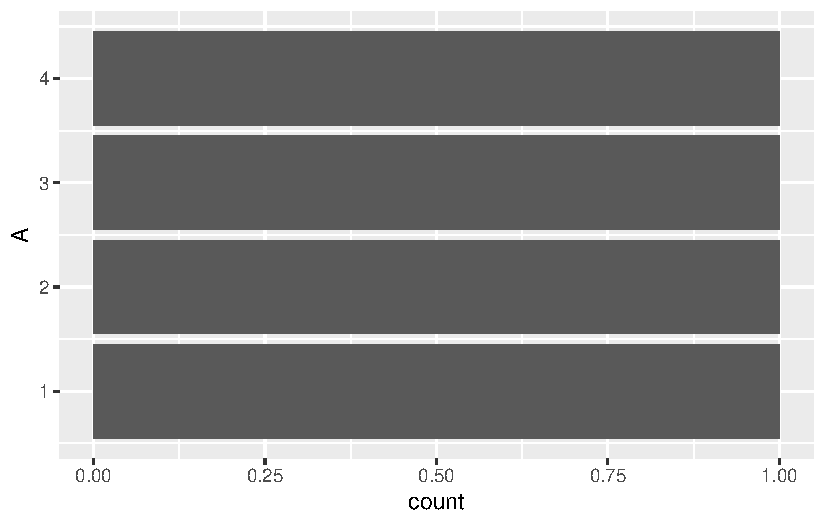
\includegraphics{Intro_to__ggplot_files/figure-pdf/unnamed-chunk-34-2.pdf}

}

\end{figure}

If the aesthetics are mapped and inherited, you can still create a plot
that accounts for both \texttt{x} and \texttt{y} variables. Passing
\texttt{stat\ =\ "identity"} to \texttt{geom\_bar()} will produce a bar
plot that presents the value of \texttt{y} in the data frame (its
identity) for each value of \texttt{x}.

When passing, pay attention to which variables are inherited by both
\texttt{x} and \texttt{y} as they will likely produce very different
plots.

\begin{Shaded}
\begin{Highlighting}[]
\NormalTok{DATA }\SpecialCharTok{\%\textgreater{}\%}
  \FunctionTok{ggplot}\NormalTok{(., }\FunctionTok{aes}\NormalTok{(}\AttributeTok{x =}\NormalTok{ A, }\AttributeTok{y =}\NormalTok{ B)) }\SpecialCharTok{+}
  \FunctionTok{geom\_bar}\NormalTok{(}\AttributeTok{stat =} \StringTok{"identity"}\NormalTok{)}
\end{Highlighting}
\end{Shaded}

\begin{figure}[H]

{\centering 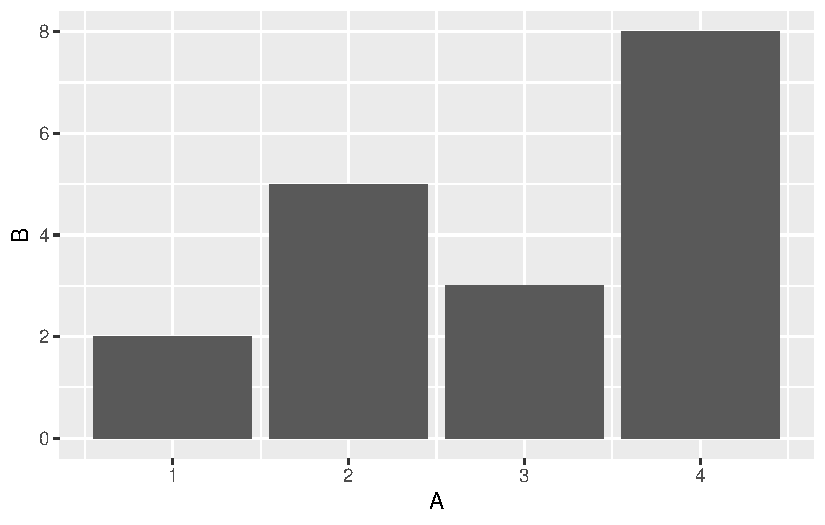
\includegraphics{Intro_to__ggplot_files/figure-pdf/unnamed-chunk-35-1.pdf}

}

\end{figure}

\begin{Shaded}
\begin{Highlighting}[]
\NormalTok{DATA }\SpecialCharTok{\%\textgreater{}\%}
  \FunctionTok{ggplot}\NormalTok{(., }\FunctionTok{aes}\NormalTok{(}\AttributeTok{x =}\NormalTok{ B, }\AttributeTok{y =}\NormalTok{ A)) }\SpecialCharTok{+}
  \FunctionTok{geom\_bar}\NormalTok{(}\AttributeTok{stat =} \StringTok{"identity"}\NormalTok{)}
\end{Highlighting}
\end{Shaded}

\begin{figure}[H]

{\centering 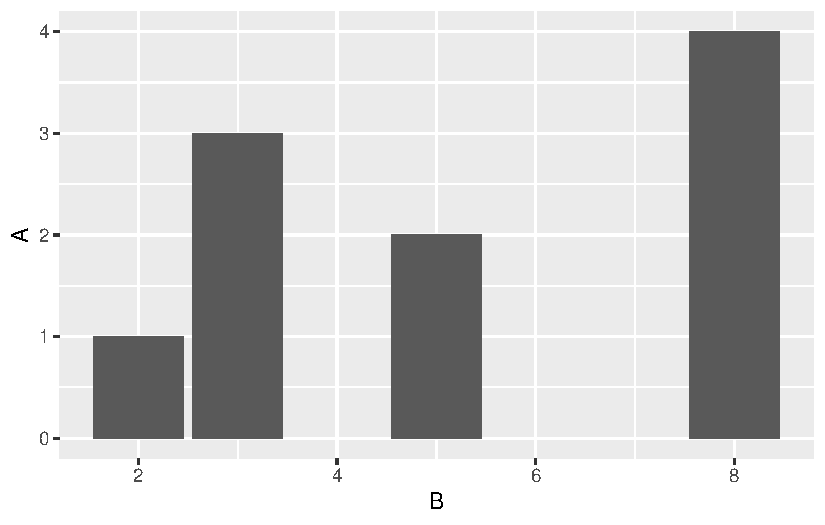
\includegraphics{Intro_to__ggplot_files/figure-pdf/unnamed-chunk-35-2.pdf}

}

\end{figure}

By default, the scale for x and y are continuous (see above). If you
don't like the fact that bars take positions for which there are no
labels and that labels are where no bars are, convert \texttt{B} it to a
factor.

\begin{Shaded}
\begin{Highlighting}[]
\NormalTok{DATA }\SpecialCharTok{\%\textgreater{}\%}
  \FunctionTok{ggplot}\NormalTok{(., }\FunctionTok{aes}\NormalTok{(}\AttributeTok{x =} \FunctionTok{as.factor}\NormalTok{(B), }\AttributeTok{y =}\NormalTok{ A)) }\SpecialCharTok{+}
  \FunctionTok{geom\_bar}\NormalTok{(}\AttributeTok{stat =} \StringTok{"identity"}\NormalTok{)}
\end{Highlighting}
\end{Shaded}

\begin{figure}[H]

{\centering 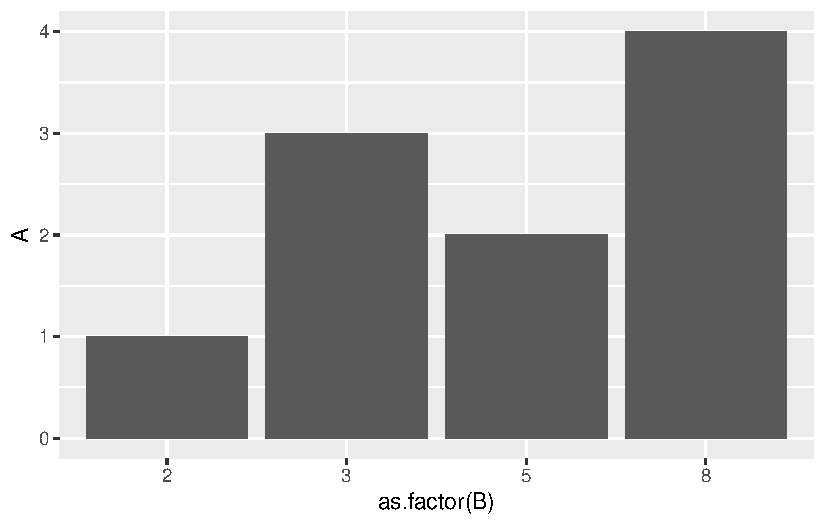
\includegraphics{Intro_to__ggplot_files/figure-pdf/unnamed-chunk-36-1.pdf}

}

\end{figure}

\hypertarget{geom_col}{%
\subsection{\texorpdfstring{\emph{\texttt{geom\_col()}}}{geom\_col()}}\label{geom_col}}

\texttt{geom\_bar(stat\ =\ "identity")} is actually the same as another
plot. A column plot using \texttt{geom\_col()}. We need both \texttt{x}
and \texttt{y} variables and when specified, the columns will plotted
for each unique level of \texttt{x} at a height corresponding to the
value of \texttt{y}. One way to think about \texttt{geom\_col()} is that
it plots columns at the same location as the points in
\texttt{geom\_point()}.

\begin{Shaded}
\begin{Highlighting}[]
\NormalTok{DATA }\SpecialCharTok{\%\textgreater{}\%}
  \FunctionTok{select}\NormalTok{(., }\FunctionTok{c}\NormalTok{(}\StringTok{"A"}\NormalTok{, }\StringTok{"B"}\NormalTok{))}
\end{Highlighting}
\end{Shaded}

\begin{verbatim}
  A B
1 1 2
2 2 5
3 3 3
4 4 8
\end{verbatim}

\begin{Shaded}
\begin{Highlighting}[]
\NormalTok{DATA }\SpecialCharTok{\%\textgreater{}\%}
  \FunctionTok{ggplot}\NormalTok{(., }\FunctionTok{aes}\NormalTok{(}\AttributeTok{x =}\NormalTok{ A, }\AttributeTok{y =}\NormalTok{ B)) }\SpecialCharTok{+}
  \FunctionTok{geom\_col}\NormalTok{()}
\end{Highlighting}
\end{Shaded}

\begin{figure}[H]

{\centering 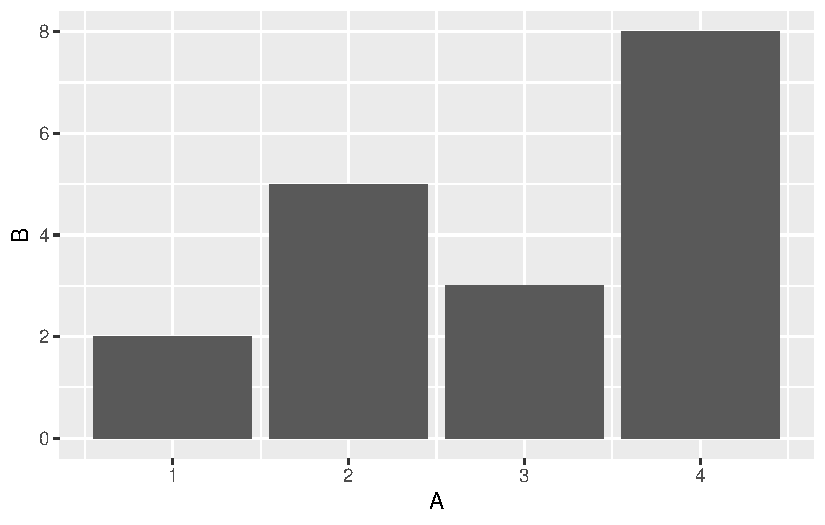
\includegraphics{Intro_to__ggplot_files/figure-pdf/unnamed-chunk-37-1.pdf}

}

\end{figure}

\begin{Shaded}
\begin{Highlighting}[]
\NormalTok{DATA }\SpecialCharTok{\%\textgreater{}\%}
  \FunctionTok{ggplot}\NormalTok{(., }\FunctionTok{aes}\NormalTok{(}\AttributeTok{x =}\NormalTok{ A, }\AttributeTok{y =}\NormalTok{ C)) }\SpecialCharTok{+}
  \FunctionTok{geom\_col}\NormalTok{()}
\end{Highlighting}
\end{Shaded}

\begin{figure}[H]

{\centering 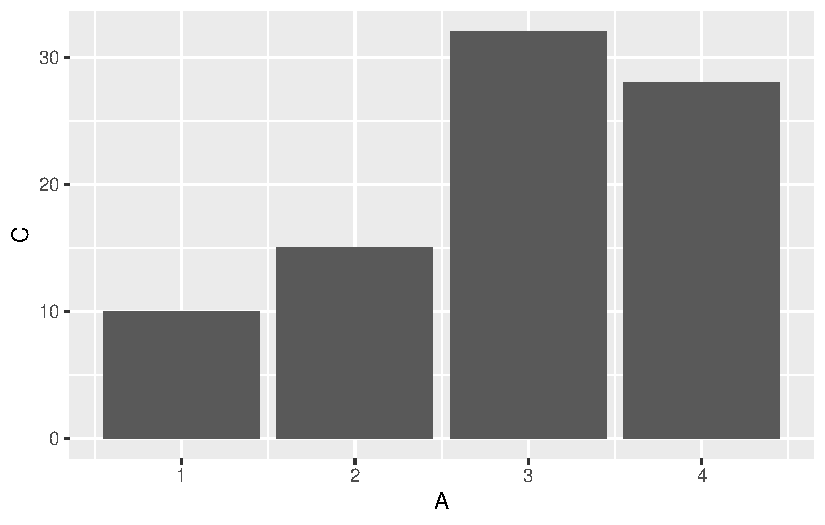
\includegraphics{Intro_to__ggplot_files/figure-pdf/unnamed-chunk-37-2.pdf}

}

\end{figure}

If your x axis (or y axis) is categorical/discrete rather than
continuous.

\begin{Shaded}
\begin{Highlighting}[]
\NormalTok{DATA }\SpecialCharTok{\%\textgreater{}\%}
  \FunctionTok{ggplot}\NormalTok{(., }\FunctionTok{aes}\NormalTok{(}\AttributeTok{x =}\NormalTok{ D, }\AttributeTok{y =}\NormalTok{ A)) }\SpecialCharTok{+} 
  \FunctionTok{geom\_col}\NormalTok{()}
\end{Highlighting}
\end{Shaded}

\begin{figure}[H]

{\centering 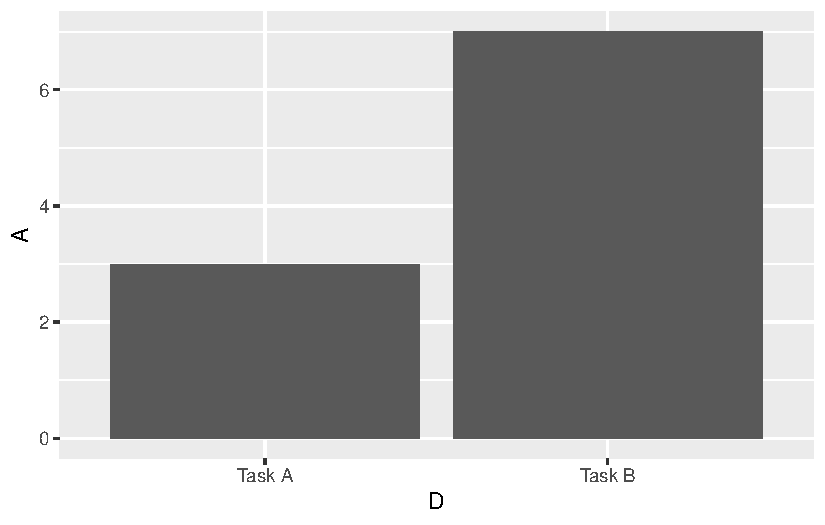
\includegraphics{Intro_to__ggplot_files/figure-pdf/unnamed-chunk-38-1.pdf}

}

\end{figure}

\begin{Shaded}
\begin{Highlighting}[]
\NormalTok{DATA }\SpecialCharTok{\%\textgreater{}\%}
  \FunctionTok{ggplot}\NormalTok{(., }\FunctionTok{aes}\NormalTok{(}\AttributeTok{x =}\NormalTok{ A, }\AttributeTok{y =}\NormalTok{ D)) }\SpecialCharTok{+} 
  \FunctionTok{geom\_col}\NormalTok{()}
\end{Highlighting}
\end{Shaded}

\begin{figure}[H]

{\centering 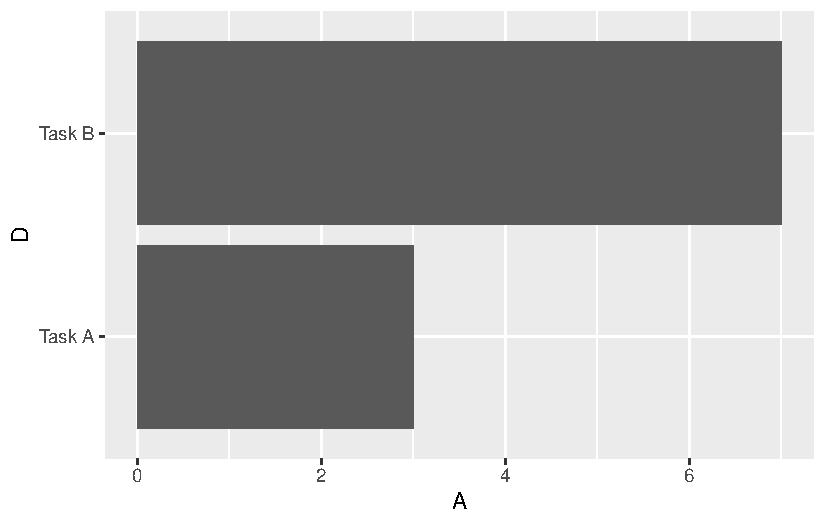
\includegraphics{Intro_to__ggplot_files/figure-pdf/unnamed-chunk-38-2.pdf}

}

\end{figure}

\hypertarget{adding-layers-to-plots}{%
\section{\texorpdfstring{\textbf{Adding Layers To
Plots}}{Adding Layers To Plots}}\label{adding-layers-to-plots}}

You can \emph{add} a layer to a plot using \texttt{+}. Unlike
\texttt{\%\textgreater{}\%}, you are not passing the object to another
function but rather you are taking the current plot object and adding to
it another layer.

For example:

\begin{Shaded}
\begin{Highlighting}[]
\NormalTok{DATA }\SpecialCharTok{\%\textgreater{}\%}
  \FunctionTok{ggplot}\NormalTok{(., }\FunctionTok{aes}\NormalTok{(}\AttributeTok{x =}\NormalTok{ A, }\AttributeTok{y =}\NormalTok{ B)) }\SpecialCharTok{+}
  \FunctionTok{geom\_col}\NormalTok{() }\SpecialCharTok{+} 
  \FunctionTok{geom\_point}\NormalTok{(}\AttributeTok{color =} \StringTok{"red"}\NormalTok{) }
\end{Highlighting}
\end{Shaded}

\begin{figure}[H]

{\centering 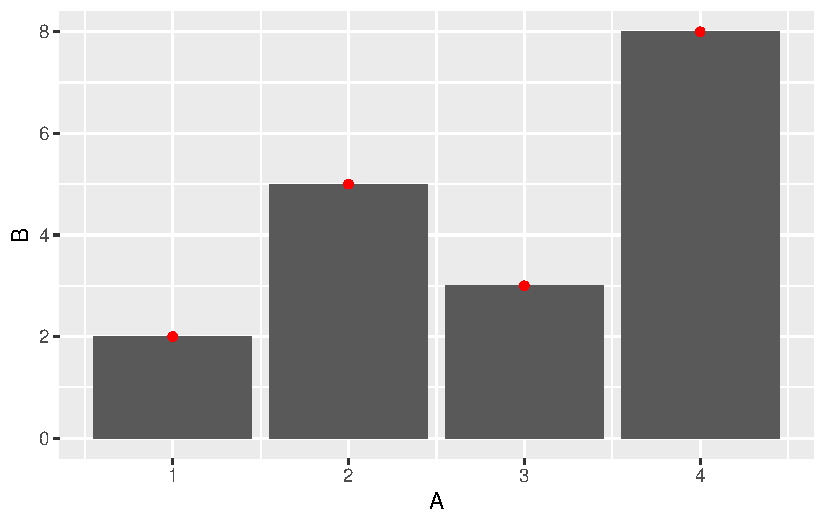
\includegraphics{Intro_to__ggplot_files/figure-pdf/unnamed-chunk-39-1.pdf}

}

\end{figure}

\hypertarget{adding-layers-that-inherit-aesthetics}{%
\subsection{\texorpdfstring{\emph{Adding layers that inherit
aesthetics}}{Adding layers that inherit aesthetics}}\label{adding-layers-that-inherit-aesthetics}}

When aesthetics are mapped to the initialized \texttt{ggplot()} object,
the \texttt{x} and \texttt{y} variables therein carry through to the
geometries. This is not a problem when the geometries are using similar
information as with \texttt{geom\_point()}, \texttt{geom\_line()}, and
even \texttt{geom\_col()}.

\begin{Shaded}
\begin{Highlighting}[]
\NormalTok{map }\OtherTok{\textless{}{-}} \FunctionTok{ggplot}\NormalTok{(}\AttributeTok{data =}\NormalTok{ DATA, }
              \AttributeTok{mapping =} \FunctionTok{aes}\NormalTok{(A, C))}

\NormalTok{map }\SpecialCharTok{+} 
  \FunctionTok{geom\_point}\NormalTok{() }\SpecialCharTok{+}
  \FunctionTok{geom\_line}\NormalTok{() }\SpecialCharTok{+}
  \FunctionTok{geom\_col}\NormalTok{()}
\end{Highlighting}
\end{Shaded}

\begin{figure}[H]

{\centering 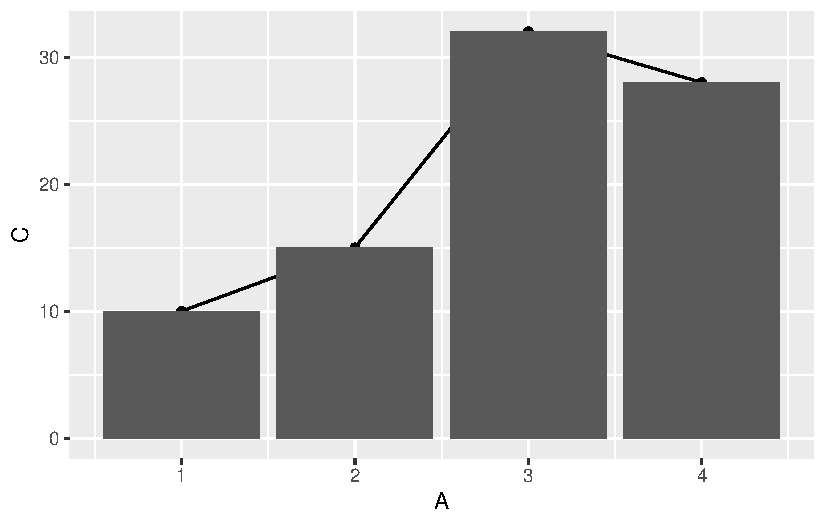
\includegraphics{Intro_to__ggplot_files/figure-pdf/unnamed-chunk-40-1.pdf}

}

\end{figure}

But because \texttt{geom\_bar()} takes only \texttt{x} or \texttt{y},
there will be a problem. Test it on your own.

\hypertarget{adding-layers-that-do-not-that-inherit-aesthetics}{%
\subsection{Adding layers that do not that inherit
aesthetics}\label{adding-layers-that-do-not-that-inherit-aesthetics}}

When aesthetics are not inherited by the initial object, they can be set
or mapped in their own geometry. This example does not even pass
\texttt{data\ =\ DATA}. If it did and each geometry used \texttt{DATA},
then that doesn't need passing. Only omitted characteristics need
mapping.

\begin{Shaded}
\begin{Highlighting}[]
\NormalTok{map }\OtherTok{\textless{}{-}} \FunctionTok{ggplot}\NormalTok{()   }

\NormalTok{map }\SpecialCharTok{+} 
  \FunctionTok{geom\_point}\NormalTok{(}\AttributeTok{data =}\NormalTok{ DATA, }
             \AttributeTok{mapping =} \FunctionTok{aes}\NormalTok{(A, C)) }\SpecialCharTok{+}
  \FunctionTok{geom\_col}\NormalTok{(}\AttributeTok{data =}\NormalTok{ DATA, }
           \AttributeTok{mapping =} \FunctionTok{aes}\NormalTok{(A, B),}
           \AttributeTok{fill =} \StringTok{"green"}\NormalTok{) }\SpecialCharTok{+}
  \FunctionTok{geom\_line}\NormalTok{(}\AttributeTok{data =}\NormalTok{ DATA, }
            \AttributeTok{mapping =} \FunctionTok{aes}\NormalTok{(A, B), }
            \AttributeTok{linetype =} \StringTok{"dashed"}\NormalTok{,}
            \AttributeTok{color =} \StringTok{"red"}\NormalTok{, }
            \AttributeTok{size =} \DecValTok{1}\NormalTok{, }
            \AttributeTok{alpha =}\NormalTok{ .}\DecValTok{5}\NormalTok{)}
\end{Highlighting}
\end{Shaded}

\begin{verbatim}
Warning: Using `size` aesthetic for lines was deprecated in ggplot2 3.4.0.
i Please use `linewidth` instead.
\end{verbatim}

\begin{figure}[H]

{\centering 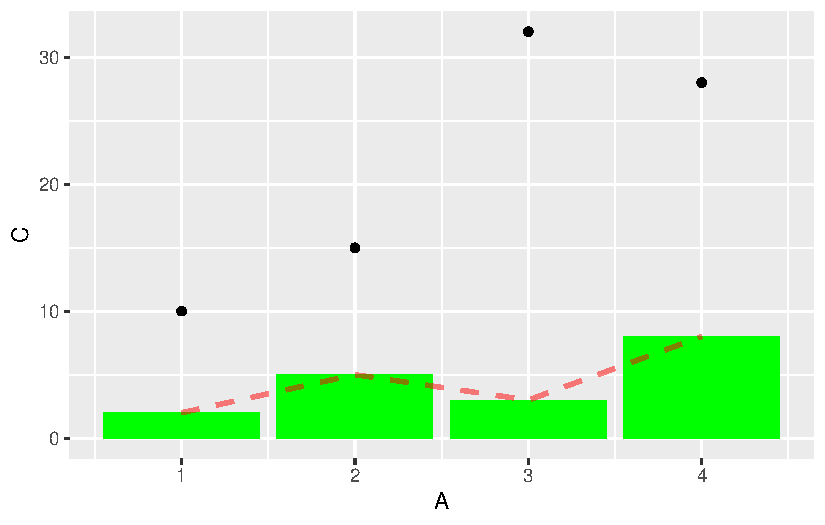
\includegraphics{Intro_to__ggplot_files/figure-pdf/unnamed-chunk-41-1.pdf}

}

\end{figure}

By specifying \texttt{DATA} and \texttt{aes(A,\ B)}, all geometries
using \texttt{DATA} with \texttt{x\ =\ A} and \texttt{y\ =\ B} will
inherit them. Otherwise, pass the necessary arguments to the geometries.

\begin{Shaded}
\begin{Highlighting}[]
\NormalTok{map }\OtherTok{\textless{}{-}} \FunctionTok{ggplot}\NormalTok{(}\AttributeTok{data =}\NormalTok{ DATA, }
              \AttributeTok{mapping =} \FunctionTok{aes}\NormalTok{(A, B))}

\NormalTok{map }\SpecialCharTok{+} 
  \FunctionTok{geom\_col}\NormalTok{(}\AttributeTok{fill =} \StringTok{"green"}\NormalTok{) }\SpecialCharTok{+}            \CommentTok{\# set all columns to blue}
  \FunctionTok{geom\_line}\NormalTok{(}\AttributeTok{mapping =} \FunctionTok{aes}\NormalTok{(}\AttributeTok{y =}\NormalTok{ C),      }\CommentTok{\# a new mapping y = C for the line data}
            \AttributeTok{linetype =} \StringTok{"dashed"}\NormalTok{) }\SpecialCharTok{+}     \CommentTok{\# set the linetype}
            
  \FunctionTok{geom\_point}\NormalTok{(}\AttributeTok{mapping =} \FunctionTok{aes}\NormalTok{(}\AttributeTok{color =}\NormalTok{ B,  }\CommentTok{\# map color to A (inherited as y)  }
                           \AttributeTok{size =}\NormalTok{ A),  }\CommentTok{\# map size to B (inherited as x)}
            \AttributeTok{alpha =}\NormalTok{ .}\DecValTok{5}                 \CommentTok{\# set alpha transparency}
\NormalTok{            ) }\SpecialCharTok{+}
  \FunctionTok{theme\_classic}\NormalTok{()}
\end{Highlighting}
\end{Shaded}

\begin{figure}[H]

{\centering 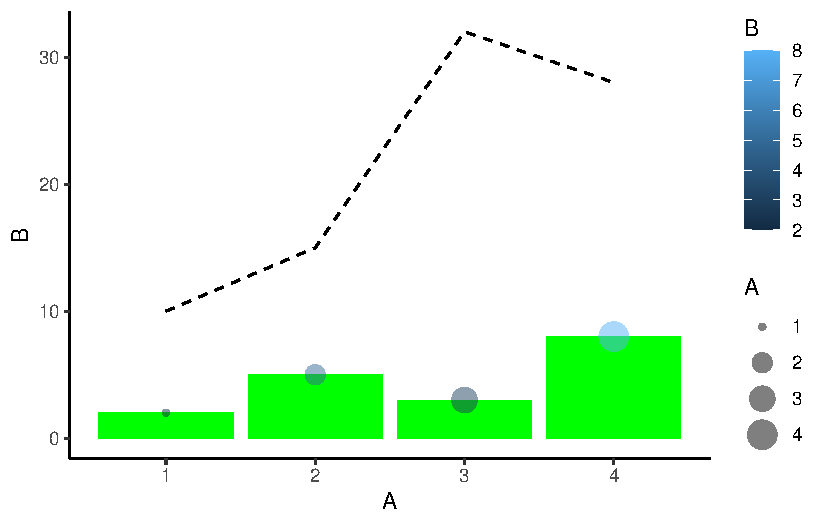
\includegraphics{Intro_to__ggplot_files/figure-pdf/unnamed-chunk-42-1.pdf}

}

\end{figure}

Now, this plot is certainly not the best and it certainly needs work.
But the coding of the plot illustrates the flexibility of ggplot for
adding plot geometry layers to a single plot, utilizing aesthetics
inherited from an initialized object, mapping new aesthetics not
inherited, setting aesthetic constants, and mapping variables to
aesthetics.

\begin{Shaded}
\begin{Highlighting}[]
 \FunctionTok{geom\_point}\NormalTok{(}\FunctionTok{aes}\NormalTok{(sugars, rating))}
\end{Highlighting}
\end{Shaded}

\begin{verbatim}
mapping: x = ~sugars, y = ~rating 
geom_point: na.rm = FALSE
stat_identity: na.rm = FALSE
position_identity 
\end{verbatim}

\hypertarget{position-adjustment-to-address-overplotting}{%
\section{\texorpdfstring{\textbf{Position Adjustment to Address
Overplotting}}{Position Adjustment to Address Overplotting}}\label{position-adjustment-to-address-overplotting}}

The plot layer we did not yet address is position. In order for a point
plot, bar plot, box plot or other plot to appear, they have to take a
position in that space. An example involving points will help
illustrate.

When plotting points on a plot, no matter what coordinate system you
plot in, an xy coordinate will take a particular position in visual
space. Following a Cartesian coordinate system, I'm sue you could
imagine visually a point on a plot at position x = 3, y = 5. A data
visualization problem occurs when two or more points also take that same
xy position. Can you imagine 2 points in that same position? How about
5? Or even 11? You see the problem.

When you have many data points in a plot, they will overlap if they
share a position, thus masking each other. When one point is hidden
behind another point, viewers cannot see that there are multiple points.
And in a worst-case scenario, those overlapping points are interpreted
as a single point, leading to incorrect data storytelling or memory for
said story. This description illustrates what is referred to as
\emph{overplotting}.

As a data storyteller, you have to deal with overplotting somehow. If
you have an audience, you could explain this problem during a talk or in
a write up. But a picture speaks a thousand words, if you let it.
Because we are on the topic of data visualization, we could just address
this overplotting issue by simply changing the position of the points
slightly using some stochastic process (won't be the same for each
plot). For an x = 3, y = 5 point, how can we change the position
slightly so it doesn't overlap with another point at the same position?
Well, maybe by adding some noise to the data, one point could be
positioned at 3.1, 5.0 and another and 3.0, 5.1, and another at 3.1,
4.9, and another at 2.9, 5.1, etc. What you might imagine is a cluster
of points around space x = 3, y = 5, each taking a slightly different
position so that they don't overlap and are all visible.

A good example of dealing with overplotting was seen in the first plot.
Without adding any noise to the data (e.g.,
\texttt{position\ =\ "jitter"}) and changing \texttt{alpha}, the
\texttt{mpg} for each cylinder level are plotted on top of each other

\begin{Shaded}
\begin{Highlighting}[]
\FunctionTok{ggplot}\NormalTok{(mtcars) }\SpecialCharTok{+}
  \FunctionTok{geom\_point}\NormalTok{(}\FunctionTok{aes}\NormalTok{(}\AttributeTok{x =} \FunctionTok{factor}\NormalTok{(cyl), }
                 \AttributeTok{y =}\NormalTok{ mpg, }
                 \AttributeTok{color =} \FunctionTok{factor}\NormalTok{(cyl))}
\NormalTok{             )}
\end{Highlighting}
\end{Shaded}

\begin{figure}[H]

{\centering 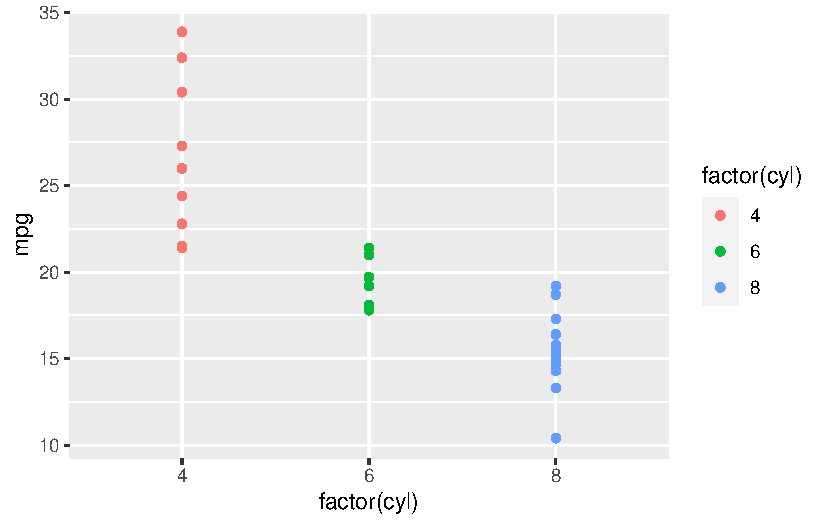
\includegraphics{Intro_to__ggplot_files/figure-pdf/unnamed-chunk-44-1.pdf}

}

\end{figure}

Changing the positioning by ``jittering'' them will make them cluster
around their levels but visibly differentiated from each other. To
facilitate the visual, we could change \texttt{alpha} to make the points
somewhat transparent such that the overlap is darkend.

\begin{Shaded}
\begin{Highlighting}[]
\FunctionTok{ggplot}\NormalTok{(mtcars) }\SpecialCharTok{+}
  \FunctionTok{geom\_point}\NormalTok{(}\FunctionTok{aes}\NormalTok{(}\AttributeTok{x =} \FunctionTok{factor}\NormalTok{(cyl), }
                 \AttributeTok{y =}\NormalTok{ mpg, }
                 \AttributeTok{color =} \FunctionTok{factor}\NormalTok{(cyl)),}
             \AttributeTok{position =} \StringTok{"jitter"}\NormalTok{, }
             \AttributeTok{alpha =}\NormalTok{ .}\DecValTok{7}
\NormalTok{             ) }
\end{Highlighting}
\end{Shaded}

\begin{figure}[H]

{\centering 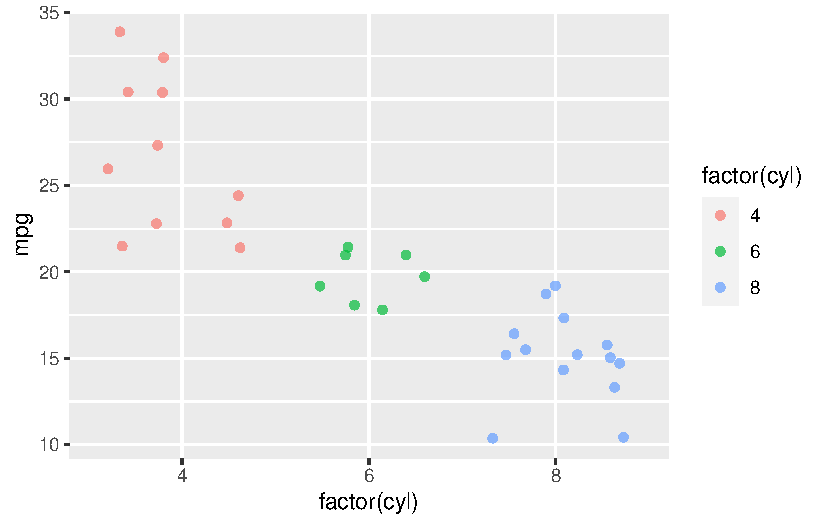
\includegraphics{Intro_to__ggplot_files/figure-pdf/unnamed-chunk-45-1.pdf}

}

\end{figure}

\hypertarget{facetting-plots}{%
\section{\texorpdfstring{\textbf{Facetting
Plots}}{Facetting Plots}}\label{facetting-plots}}

When you want to plot the same data separately for levels or variations
in another variable, you can plot facets. Using \texttt{facet\_wrap()},
we can pass the \texttt{D} variable like this:
\texttt{facet\_wrap(\textasciitilde{}D)}

\begin{Shaded}
\begin{Highlighting}[]
\NormalTok{DATA }\SpecialCharTok{\%\textgreater{}\%}
  \FunctionTok{ggplot}\NormalTok{() }\SpecialCharTok{+}
  \FunctionTok{geom\_col}\NormalTok{(}\AttributeTok{mapping =} \FunctionTok{aes}\NormalTok{(A, B),}
           \AttributeTok{fill =} \StringTok{"green"}\NormalTok{) }\SpecialCharTok{+}
  \FunctionTok{facet\_wrap}\NormalTok{(}\SpecialCharTok{\textasciitilde{}}\NormalTok{D)}
\end{Highlighting}
\end{Shaded}

\begin{figure}[H]

{\centering 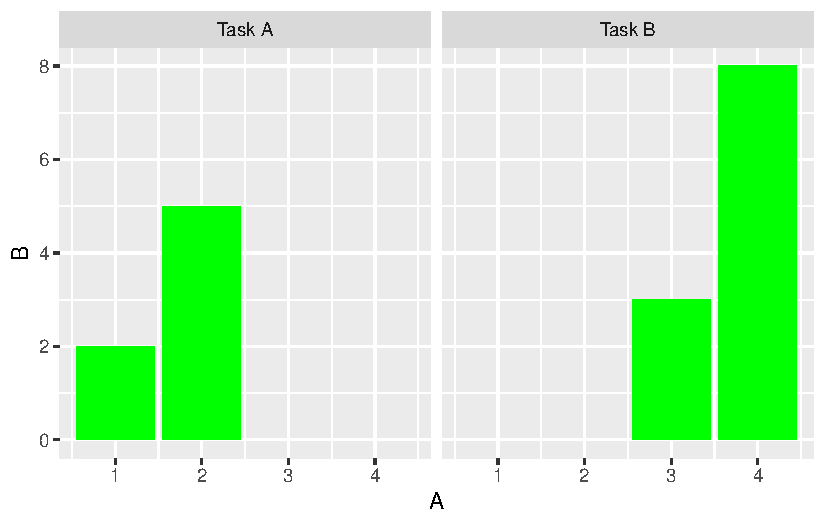
\includegraphics{Intro_to__ggplot_files/figure-pdf/unnamed-chunk-46-1.pdf}

}

\end{figure}

Unfortunately, with this small data set, values differ in \texttt{A}
based on \texttt{D} (the task) so you might be confused. Rest assured
the function is doing what it should. Our data only have responses 1 and
2 for Task A and 3 and 4 for Task B. Perhaps a better illustration is
with \texttt{mtcars} data. A point plot visualizing \texttt{wt} and
\texttt{mpg} for each cylinder size.

\begin{Shaded}
\begin{Highlighting}[]
\NormalTok{mtcars }\SpecialCharTok{\%\textgreater{}\%}
  \FunctionTok{ggplot}\NormalTok{() }\SpecialCharTok{+}
  \FunctionTok{geom\_point}\NormalTok{(}\AttributeTok{mapping =} \FunctionTok{aes}\NormalTok{(wt, mpg),}
             \AttributeTok{fill =} \StringTok{"green"}\NormalTok{) }\SpecialCharTok{+}
  \FunctionTok{facet\_wrap}\NormalTok{(}\SpecialCharTok{\textasciitilde{}}\NormalTok{cyl)}
\end{Highlighting}
\end{Shaded}

\begin{figure}[H]

{\centering \includegraphics{Intro_to__ggplot_files/figure-pdf/unnamed-chunk-47-1.pdf}

}

\end{figure}

\hypertarget{troubleshooting-passing-vectors}{%
\section{\texorpdfstring{\textbf{Troubleshooting Passing
Vectors}}{Troubleshooting Passing Vectors}}\label{troubleshooting-passing-vectors}}

You may sometimes have a data set that has many variables containing
special characters. In such cases, you may try to pass as arguments to
the \texttt{x} and \texttt{y} aesthetics (viz., \texttt{aes()}) the
variable names in quotes. If so, \texttt{ggplot2} will plot a single
point (rather than all xy coordinates).

Let's see using the \texttt{mtcars} data to plot car weight against
miles per gallon.

\begin{Shaded}
\begin{Highlighting}[]
\NormalTok{mtcars }\SpecialCharTok{\%\textgreater{}\%}
    \FunctionTok{ggplot}\NormalTok{(., }
       \FunctionTok{aes}\NormalTok{(}\AttributeTok{x =} \StringTok{"mpg"}\NormalTok{, }\AttributeTok{y =} \StringTok{"wt"}\NormalTok{)) }\SpecialCharTok{+} \FunctionTok{geom\_point}\NormalTok{()}
\end{Highlighting}
\end{Shaded}

\begin{figure}[H]

{\centering \includegraphics{Intro_to__ggplot_files/figure-pdf/unnamed-chunk-48-1.pdf}

}

\end{figure}

This is certainly awkward. You may not even think to just pass the name
without quotes but if you did, you would see a nice scatter plot.

\begin{Shaded}
\begin{Highlighting}[]
\NormalTok{mtcars }\SpecialCharTok{\%\textgreater{}\%}
    \FunctionTok{ggplot}\NormalTok{(., }
       \FunctionTok{aes}\NormalTok{(}\AttributeTok{x =}\NormalTok{ mpg, }\AttributeTok{y =}\NormalTok{ wt)) }\SpecialCharTok{+} \FunctionTok{geom\_point}\NormalTok{()}
\end{Highlighting}
\end{Shaded}

\begin{figure}[H]

{\centering \includegraphics{Intro_to__ggplot_files/figure-pdf/unnamed-chunk-49-1.pdf}

}

\end{figure}

Easy fix if you know what you are doing but there is a larger problem
when you have special characters in variable names.

\begin{Shaded}
\begin{Highlighting}[]
\CommentTok{\#add new vars}
\NormalTok{mtcars2 }\OtherTok{\textless{}{-}}\NormalTok{ mtcars }\SpecialCharTok{\%\textgreater{}\%}
  \FunctionTok{mutate}\NormalTok{(., }
         \StringTok{"\_wt"} \OtherTok{=}\NormalTok{ wt,}
         \StringTok{"\_mpg"} \OtherTok{=}\NormalTok{ mpg)}
\end{Highlighting}
\end{Shaded}

This code will produce an error, which unfortunately is not very
diagnostic regarding the unexpected symbol. There is no quote in the
code but the error seems to be stating there are \texttt{"} which are
causing problems.

\texttt{mtcars2\ \%\textgreater{}\%} \texttt{ggplot(.,}
\texttt{aes(x\ =\ \_mpg,\ y\ =\ \_wt))\ +\ geom\_point()}

So what do you do?

You can use the tick (e.g., ```'') to wrap your variable names, though
this approach may never come to mind unless you work with RStudio long
enough to see that the tick is often wrapped around variable names.
Nevertheless, this will solve your problem.

\begin{Shaded}
\begin{Highlighting}[]
\NormalTok{mtcars2 }\SpecialCharTok{\%\textgreater{}\%}
    \FunctionTok{ggplot}\NormalTok{(., }
       \FunctionTok{aes}\NormalTok{(}\AttributeTok{x =}\NormalTok{ .data}\SpecialCharTok{$}\StringTok{\textasciigrave{}}\AttributeTok{\_mpg}\StringTok{\textasciigrave{}}\NormalTok{, }\AttributeTok{y =}\NormalTok{ .data}\SpecialCharTok{$}\StringTok{\textasciigrave{}}\AttributeTok{\_wt}\StringTok{\textasciigrave{}}\NormalTok{)) }\SpecialCharTok{+} \FunctionTok{geom\_point}\NormalTok{()}
\end{Highlighting}
\end{Shaded}

\begin{figure}[H]

{\centering \includegraphics{Intro_to__ggplot_files/figure-pdf/unnamed-chunk-51-1.pdf}

}

\end{figure}

Another approach if you are using \texttt{\%\textgreater{}\%}, the
\texttt{.data} pronoun as part of the \texttt{tidyverse} will allow you
to pass the quoted name as a the argument by putting it in double square
brackets (e.g., \texttt{{[}{[}{]}{]}})

To see how single or double brackets work on a data frame, both are
applied below to the \texttt{mtcars2} data frame containing the new
variables.

\begin{Shaded}
\begin{Highlighting}[]
\NormalTok{mtcars2[}\StringTok{"\_mpg"}\NormalTok{]}
\end{Highlighting}
\end{Shaded}

\begin{verbatim}
                    _mpg
Mazda RX4           21.0
Mazda RX4 Wag       21.0
Datsun 710          22.8
Hornet 4 Drive      21.4
Hornet Sportabout   18.7
Valiant             18.1
Duster 360          14.3
Merc 240D           24.4
Merc 230            22.8
Merc 280            19.2
Merc 280C           17.8
Merc 450SE          16.4
Merc 450SL          17.3
Merc 450SLC         15.2
Cadillac Fleetwood  10.4
Lincoln Continental 10.4
Chrysler Imperial   14.7
Fiat 128            32.4
Honda Civic         30.4
Toyota Corolla      33.9
Toyota Corona       21.5
Dodge Challenger    15.5
AMC Javelin         15.2
Camaro Z28          13.3
Pontiac Firebird    19.2
Fiat X1-9           27.3
Porsche 914-2       26.0
Lotus Europa        30.4
Ford Pantera L      15.8
Ferrari Dino        19.7
Maserati Bora       15.0
Volvo 142E          21.4
\end{verbatim}

\begin{Shaded}
\begin{Highlighting}[]
\NormalTok{mtcars2[[}\StringTok{"\_mpg"}\NormalTok{]]}
\end{Highlighting}
\end{Shaded}

\begin{verbatim}
 [1] 21.0 21.0 22.8 21.4 18.7 18.1 14.3 24.4 22.8 19.2 17.8 16.4 17.3 15.2 10.4
[16] 10.4 14.7 32.4 30.4 33.9 21.5 15.5 15.2 13.3 19.2 27.3 26.0 30.4 15.8 19.7
[31] 15.0 21.4
\end{verbatim}

OK, and for \texttt{ggplot2}\ldots{}

\begin{Shaded}
\begin{Highlighting}[]
\NormalTok{mtcars2 }\SpecialCharTok{\%\textgreater{}\%}
    \FunctionTok{ggplot}\NormalTok{(., }
       \FunctionTok{aes}\NormalTok{(}\AttributeTok{x =}\NormalTok{ .data[[}\StringTok{"\_mpg"}\NormalTok{]], }\AttributeTok{y =}\NormalTok{ .data[[}\StringTok{"\_wt"}\NormalTok{]])) }\SpecialCharTok{+} \FunctionTok{geom\_point}\NormalTok{()}
\end{Highlighting}
\end{Shaded}

\begin{figure}[H]

{\centering \includegraphics{Intro_to__ggplot_files/figure-pdf/unnamed-chunk-53-1.pdf}

}

\end{figure}

Note: You could use \texttt{.} instead of \texttt{.data} to represent
the data frame being passed but that is discouraged and may be
deprecated (no longer work).

As a general tip when cleaning up variable names, change variables so
that they don't contain characters like ``-'' or ``\$'' or others that
don't work kindly with some functions. Using ``\_'' is fine except when
putting that at the beginning or end of variable name.

\hypertarget{setting-themes-for-plot-consistency}{%
\section{\texorpdfstring{\textbf{Setting Themes for Plot
Consistency}}{Setting Themes for Plot Consistency}}\label{setting-themes-for-plot-consistency}}

Although you can modify the plot theme by adding it as a layer, doing so
may be redundant when you do not wish to accept the default theme.
Rather that add a theme layer to your plot using
\texttt{theme\_minimal()}, \texttt{theme\_classic()}, or some other
theme, you could set the theme at the top of your code file using
\texttt{theme\_set()}. Then, all plots in the file will adhere to that
theme unless you add a layer to change it.

To set the theme to \texttt{theme\_minimal()}, pass that theme into
\texttt{theme\_set()}. We will often use a theme from the \texttt{see}
library, \texttt{see::theme\_modern()}. If set here, all plots after,
and only after, setting the theme will abide by those theme
characteristics.

\begin{Shaded}
\begin{Highlighting}[]
\FunctionTok{theme\_set}\NormalTok{(}\FunctionTok{theme\_minimal}\NormalTok{())}

\CommentTok{\#theme\_set(see::theme\_modern())}
\end{Highlighting}
\end{Shaded}




\end{document}
